%%
%% The original source files were:
%%
%% samples.dtx  (with options: `all,proceedings,bibtex,manuscript')
%% 
%% IMPORTANT NOTICE:
%% 
%% For the copyright see the source file.
%% 
%% Any modified versions of this file must be renamed
%% with new filenames distinct from sample-manuscript.tex.
%% 
%% For distribution of the original source see the terms
%% for copying and modification in the file samples.dtx.
%% 
%% This generated file may be distributed as long as the
%% original source files, as listed above, are part of the
%% same distribution. (The sources need not necessarily be
%% in the same archive or directory.)
%%
%%
%% Commands for TeXCount
%TC:macro \cite [option:text,text]
%TC:macro \citep [option:text,text]
%TC:macro \citet [option:text,text]
%TC:envir table 0 1
%TC:envir table* 0 1
%TC:envir tabular [ignore] word
%TC:envir displaymath 0 word
%TC:envir math 0 word
%TC:envir comment 0 0
%%
%% The first command in your LaTeX source must be the \documentclass
%% command.
%%
%% For submission and review of your manuscript please change the
%% command to \documentclass[manuscript, screen, review]{acmart}.
%%
%% When submitting camera ready or to TAPS, please change the command
%% to \documentclass[sigconf]{acmart} or whichever template is required
%% for your publication.
%%
%%
\documentclass[manuscript,screen,review]{acmart}


\usepackage{algorithm}
% Use algorithmicx + algpseudocode: provides \Require, \Ensure, \State, and \Comment
\usepackage{algorithmicx}
\usepackage{algpseudocode}
% Provide compatibility shims for uppercase macros used in the document
% Some authors use \REQUIRE/\ENSURE/\UPON/\ENDUPON (uppercase) — map them to algpseudocode
\providecommand{\REQUIRE}[1]{\Require{#1}}
\providecommand{\ENSURE}[1]{\Ensure{#1}}
% \UPON{<cond>} will render as a bold 'Upon <cond>' state line inside algorithmic blocks
\providecommand{\UPON}[1]{\State\textbf{Upon}~#1}
\providecommand{\ENDUPON}{}
% Provide uppercase aliases commonly used in algorithm blocks
\providecommand{\STATE}{\State}
\providecommand{\COMMENT}[1]{\Comment{#1}}
% Map common uppercase algorithmic keywords to algorithmicx/algpseudocode commands
\providecommand{\IF}{\If}
\providecommand{\ELSE}{\Else}
\providecommand{\ELSIF}{\ElsIf}
\providecommand{\ENDIF}{\EndIf}
\providecommand{\FOR}{\For}
\providecommand{\ENDFOR}{\EndFor}
\providecommand{\WHILE}{\While}
\providecommand{\ENDWHILE}{\EndWhile}
\providecommand{\RETURN}{\State\textbf{return}~}
% color support for \textcolor used inside algorithms
\usepackage{xcolor}
% Math packages required for \text and bold symbols inside math
\usepackage{amsmath}
\usepackage{bm}
% Define common math operators used in the document
\DeclareMathOperator*{\argmin}{arg\,min}
\DeclareMathOperator*{\argmax}{arg\,max}
\usepackage{multirow}
% Enable list customization (leftmargin, itemsep, etc.) used in the document
\usepackage{enumitem}
% Ensure header height is sufficient for fancyhdr
\setlength{\headheight}{20.48303pt}
% theorem environments used in the document
% acmart/amsart already provides amsthm; do not load amsthm again
\newtheorem{assumption}{假设}
\newtheorem{problem}{问题}
\renewcommand{\proofname}{证明}
\AtEndPreamble{%
  \let\proposition\relax
  \let\endproposition\relax
  \newtheorem{proposition}[theorem]{命题}%
}
% 中文初稿：请用 XeLaTeX 编译
\usepackage{xeCJK}
\setCJKmainfont{SimSun}[BoldFont=SimHei]
\setCJKsansfont{SimHei}
\xeCJKsetup{PunctStyle=kaiming}

%%
%% \BibTeX command to typeset BibTeX logo in the docs
\AtBeginDocument{%
  \providecommand\BibTeX{{%
    Bib\TeX}}}

%% Rights management information.  This information is sent to you
%% when you complete the rights form.  These commands have SAMPLE
%% values in them; it is your responsibility as an author to replace
%% the commands and values with those provided to you when you
%% complete the rights form.
\setcopyright{acmlicensed}
\copyrightyear{2026}
\acmYear{2026}
\acmDOI{XXXXXXX.XXXXXXX}

%% These commands are for a PROCEEDINGS abstract or paper.
%%  \acmConference[Conference acronym 'XX]{Make sure to enter the correct
%% 	conference title from your rights confirmation email}{June 03--05,
%% 	2018}{Woodstock, NY}

%%
%%  Uncomment \acmBooktitle if the title of the proceedings is different
%%  from ``Proceedings of ...''!
%%
%%\acmBooktitle{Woodstock '18: ACM Symposium on Neural Gaze Detection,
%%  June 03--05, 2018, Woodstock, NY}
%%\acmISBN{978-1-4503-XXXX-X/2018/06}


%%
%% Submission ID.
%% Use this when submitting an article to a sponsored event. You'll
%% receive a unique submission ID from the organizers
%% of the event, and this ID should be used as the parameter to this command.
%%\acmSubmissionID{123-A56-BU3}

%%
%% For managing citations, it is recommended to use bibliography
%% files in BibTeX format.
%%
%% You can then either use BibTeX with the ACM-Reference-Format style,
%% or BibLaTeX with the acmnumeric or acmauthoryear sytles, that include
%% support for advanced citation of software artefact from the
%% biblatex-software package, also separately available on CTAN.
%%
%% Look at the sample-*-biblatex.tex files for templates showcasing
%% the biblatex styles.
%%

%%
%% The majority of ACM publications use numbered citations and
%% references.  The command \citestyle{authoryear} switches to the
%% "author year" style.
%%
%% If you are preparing content for an event
%% sponsored by ACM SIGGRAPH, you must use the "author year" style of
%% citations and references.
%% Uncommenting
%% the next command will enable that style.
%%\citestyle{acmauthoryear}


%%
%% end of the preamble, start of the body of the document source.
\begin{document}

%%
%% The "title" command has an optional parameter,
%% allowing the author to define a "short title" to be used in page headers.
\title[离散事件注入攻击检测]{基于时序半马尔可夫与参考模型可行性约束的工业离散事件注入攻击检测}
\subtitle{Timed Semi-Markov Consistency and Reference-Model Constraints for Detecting Injection Attacks on Discrete Industrial Event Streams}

%%
%% The "author" command and its associated commands are used to define
%% the authors and their affiliations.
%% Of note is the shared affiliation of the first two authors, and the
%% "authornote" and "authornotemark" commands
%% used to denote shared contribution to the research.
\author{Qi Yu}
%%\authornote{.}
%%\authornotemark[1]
\email{230240012@seu.edu.cn}
%%\orcid{1234-5678-9012}
\affiliation{%
	\institution{School of Cyber Science and Engineering, Southeast University}
	\city{Nanjing}
	\state{Jiangsu}
	\country{PR China}
}


\author{Wei Li}
%%\orcid{1234-5678-9012}
\email{xchlw@seu.edu.cn}
\authornote{corresponding author}
%%\authornotemark[1]
\affiliation{%
	\institution{School of Computer Science and Engineering, Southeast University}
	\city{Nanjing}
	\state{Jiangsu}
	\country{PR China}
}


%%
%% By default, the full list of authors will be used in the page
%% headers. Often, this list is too long, and will overlap
%% other information printed in the page headers. This command allows
%% the author to define a more concise list
%% of authors' names for this purpose.
%%\renewcommand{\shortauthors}{Qi et al.}

%%
%% The abstract is a short summary of the work to be presented in the
%% article.
\begin{abstract}
工业信息物理生产系统中，现场设备以离散活动事件（资源、操作、时间戳、作业实例）上报运行过程。攻击者在上行链路上注入或重放这些事件，即可使日志记录的状态轨迹与物理过程脱节。
仅依赖标签预测与自适应阈值的检测族，在零误报约束下对标签自洽的注入不存在可标记集合：其能够标记的转移，恰为参考模型可行性掩码已以零代价拒绝的那一部分。
既有检测工作并未覆盖这一事件层：生产线计时自动机为规避状态空间爆炸，按网络拓扑将系统分解为相互独立的顺序组件，检测在单个自动机上完成，跨组件可行性约束被主动舍弃；TABOR 将计时自动机与贝叶斯网络组合，但依赖关系被限制在同一工段之内，且显式忽略命令数据；半马尔可夫与基于计时的检测虽已对停留时长建模，却无法区分日志中``未曾观测''与参考模型``不允许''；DCTA 等报文层状态机约束的是协议会话，而非工艺参考模型与活动语义。
为此，本文将合法行为建模为带停留时长的半马尔可夫过程，以工艺参考模型导出的可行性掩码构成硬约束层，对不可行事件直接否决，并检查完成事件在同一日志中是否存在对应的指派记录；时序通道与结构通道分别经共形预测校准后并行判决，再由 CUSUM 对分级证据作序贯累积。共形保证仅在可交换口径下成立，部署阶段按时间序划分报告经验误报率。
在该设定下，攻击者为伪造更短停留所须付出的相对提前量存在闭式上界 $\rho^*(\alpha,\sigma)$---该结论是隐蔽攻击基本极限这一已有命题形式在离散事件、无系统矩阵条件下的实例。安全目标因此是``可检出，或伪造提前量有界''，而非全部检出。
公开活动日志不含注入标注。本文在 Fischertechnik Trier 真实产线事件日志上按可复现协议合成攻击，并在同一误报预算下，与按原文结构约束复现的计时自动机、TABOR 式方法、半马尔可夫似然以及参考模型符合度（违反掩码即告警）进行对照：主要检测对象是物理不可行注入与标签未改的停留时长错位；对渐变漂移，本文方法相对仅标签检测族取得结构性非零检出；对提前完成重放，检出率保持非零，但增益小于渐变漂移，本文不据此宣称显著领先；符合度代理可覆盖不可行注入，对纯时长攻击的检出为零。
\end{abstract}

\begin{CCSXML}
<ccs2012>
   <concept>
       <concept_id>10002978.10003006.10003013</concept_id>
       <concept_desc>Security and privacy~Intrusion detection systems</concept_desc>
       <concept_significance>500</concept_significance>
       </concept>
   <concept>
       <concept_id>10010520.10010521</concept_id>
       <concept_desc>Computer systems organization~Embedded and cyber-physical systems</concept_desc>
       <concept_significance>300</concept_significance>
       </concept>
</ccs2012>
\end{CCSXML}

\ccsdesc[500]{Security and privacy~Intrusion detection systems}
\ccsdesc[300]{Computer systems organization~Embedded and cyber-physical systems}

\begin{keywords}
注入攻击检测, 离散事件日志, 半马尔可夫过程, 可行性约束,
共形预测, 序贯检验, 信息物理生产系统
\end{keywords}

\maketitle


%=============================================================================
\section{引言}
\label{sec:intro}

\subsection{研究背景与动机}
\label{sec:intro_bg}

信息物理生产系统（cyber-physical production system, CPPS）中，现场设备以离散活动事件上报运行过程：一条事件含资源、操作（或状态标签）、时间戳与作业实例~\cite{monostori2016cpps,seiger2022factory}。例如，调度系统向搬运设备下达``前往某工位''的指派后，日志依次记录指派、开始执行与完成；本文检测的是这些事件是否被注入或重放，而不评测调度器随后如何改派下一任务。攻击者无须改写连续控制律或攻破设备固件，只需在上行链路上\textbf{注入或重放这些事件}，即可使日志记录的轨迹与物理过程脱节。工业信息物理系统上的检测文献主要集中于过程物理量、边界防护与网络流量~\cite{kayan2022icps}，带生命周期的活动事件很少被单独视为注入对象。典型手法是在活动尚未完成时重放``已完成''事件：单条记录在标签层面完全合法，却改写了停留时长与后继事件的上下文。若检测器仅比较预测标签与观测标签之间的几何或概率距离，则此类注入与良性众数转移不可区分：该距离是 $(\text{前驱},\text{标签})$ 的确定性函数，与该条记录为良性还是伪造无关；在零误报约束下，其可标记集合恰为可行性掩码中的零概率转移。

该攻击面之所以可被利用，是因为同一条事件流同时具备三类结构：它们可供检测器使用，而攻击者难以同时伪造。第一，工艺流程规定了哪台资源允许执行哪个操作、可由哪个前驱到达，这些可行性约束由参考过程模型给出，无法从运行日志中学习得到---日志只能给出历史上出现过的组合，无法区分``未曾观测''与``不允许''。第二，活动消耗物理时间：标签序列合法但耗时错位的事件，在纯标签模型下的概率接近于~$1$，原理上不可检测。第三，完成事件本应对应同一日志中的指派（或开始）事件；缺少前置指派的完成事件构成一步即可判定的因果缺失。产线中还存在物料流等跨资源耦合，它们表明离散事件日志不同于水处理等单过程标签流，但本文并不将令牌守恒作为统计检测通道。该日志的下游消费方式（监控、执行或派工）不在本文评测范围之内。

\subsection{与已有工作的差距}
\label{sec:intro_gap}

既有工作并未覆盖上述结构，原因并不在于其``未涉及多设备场景''，而在于其方法论前提将参考模型可行性与命令--事件配对排除在外。生产线计时自动机~\cite{maier2011timed}虽面向多模块产线，却先按网络拓扑将系统分解为相互独立的顺序组件，再在单个自动机上检查符号、时间区间与转移频率；学习并行结构的目的是规避状态空间爆炸，跨组件可行性因此被主动舍弃，检测算法也不执行跨组件一致性检查。TABOR~\cite{lin2018tabor}将计时自动机与贝叶斯网络组合，形式上似已覆盖时序与依赖，但其贝叶斯网络被限制在同一工段之内，并且显式忽略网络与命令数据，因而既无指派--完成配对，也无法表达参考模型给出的跨设备可行性。SWaT 官方攻击分类中本已包含跨阶段攻击~\cite{goh2016swat,lin2018tabor}，表明该领域已承认此类威胁的存在，但检测模型中并无与之对应的结构。DCTA~\cite{barsha2024dcta}把异常分为单报文、报文序列与时间三类，命名上与多通道划分相近，其约束对象却是智能电网 {SCADA} 的 {IEC-104} 会话，与工艺流程和活动语义无关。另一支文献处理连续控制层上的定位、编队与抗重放，对象是位置与速度估计~\cite{elsisi2023agv,mo2009replay}，同样不是离散活动事件。文献定位见第~\ref{sec:related}~节。

\subsection{本文方法}
\label{sec:intro_method}

因此，仅将``为马尔可夫模型引入时间维度''视为创新并不成立：计时自动机已用于生产线与 {SCADA} 的时序异常检测~\cite{maier2011timed,lin2018timing}，半马尔可夫对停留时长的建模亦属成熟做法~\cite{tan2008hsmm}。计时自动机的时钟守卫是区间型二值判断，落在守卫内部的小幅提前上报会被接受；半马尔可夫给出的是停留时长的概率分布，同向残差可以在序贯检验中累积。更关键的差异在可行性一侧：数据驱动模型将训练折中未出现的活动组合判为异常，会把新产品变体误判为攻击；参考模型则将``未曾观测''与``不允许''区分开。本文以参考模型给出的可行性掩码作为硬约束层的直接否决依据，以分布型停留时长作为时序通道的建模机理，而不再叠加一条从日志中学习得到的互锁统计通道。

\subsection{主要结果}
\label{sec:intro_results}

主表在 $\alpha=0.01$、延迟预算 $10$ 条并扣除偶然告警基线的口径下给出，本文不宣称全面优于既有方法。证据最充分的两项是：{A2} 由一元能力集覆盖（净检出 $0.95$），以及 {A5} 相对仅标签检测族取得结构性非零检出（$0.87$ 对 $0.00$）。{A3} 的检出率保持非零（$0.18{\pm}0.01$），增益小于渐变漂移，其机理是分布型左尾残差可被序贯累积，而非大幅领先。{A4}/{A6} 低于仅标签消融，是三路通道均分误报预算的代价，本文不将其列为优势。规避检测的相对提前量存在上界 $\rho^*(\alpha,\sigma)$；实验验证的是单次注入下的混合功效曲线。共形覆盖保证仅在可交换口径下成立，部署阶段报告时间序经验误报率。细节见第~\ref{sec:experiments}~节。

\subsection{贡献}
\label{sec:intro_contrib}

本文的贡献如下。
\begin{enumerate}
\item \textbf{把离散工业事件流上的注入检测表述为一个独立问题。}
检测对象是带生命周期的活动事件：例如调度系统向现场设备下达一项作业指派后，日志依次记录指派、开始与完成；本文检测这些记录是否被注入或重放，而不评测调度器据此如何重新派工。检测对象既不是连续控制层，也不是单一工艺过程量或网络报文会话，而主要针对参考模型不可行的注入，以及标签合法但停留时长错位的注入。
\item \textbf{以参考模型可行性掩码作为硬约束；指派--完成配对是硬约束层的第三项，本文不单独评估。}
一元能力集覆盖全部消息且良性违反率为零，这是硬约束层的主要证据。依据同一日志中的指派事件，可以拒绝缺少前置指派的完成事件；六类注入中没有专门破坏该配对关系的攻击族，故本文不将其作为与掩码并列的实验主张。二者均无法从日志中学习得到。若将符合度直接用作检测器、以违反掩码作为告警规则，则其判决与硬约束层重合。
\item \textbf{用按 $(\text{资源},\text{操作})$ 分组的分布型停留核，并以共形预测作为可交换口径下的校准手段。}
时序通道与结构通道经校准后并行判决，并由 {CUSUM} 序贯累积。相对于区间守卫，落在区间内侧的提前上报仍可被累积。部署阶段只能按时间序划分数据，共形的覆盖保证不再自动成立，误报率按时间序经验值报告，见第~\ref{sec:boundary}~节。与隐半马尔可夫基线的另一差别在于，左尾检验绑定在 $(\text{资源},\text{操作})$ 分组上，而非绑定在隐状态上。
\item \textbf{给出规避检测的相对提前量上界 $\rho^*(\alpha,\sigma)$，并指出仅标签阈值族的不可能性。}
该上界仅依赖时序变异、误报预算与重复次数，是隐蔽攻击基本极限~\cite{liu2022limits}在离散事件、无系统矩阵条件下的实例。对标签自洽的注入，预测加自适应阈值的检测族不提供超出可行性掩码的增量。
\end{enumerate}

后文组织如下。第~\ref{sec:related}~节按层次回顾相关工作并给出定位。第~\ref{sec:problem}~节给出问题描述、建模假设、威胁模型与检测问题。第~\ref{sec:framework}~节阐述硬约束层否决、时序通道与结构通道。第~\ref{sec:theory}~节先给出仅标签阈值族的不可能性，再说明分布型时长相对时钟守卫的差异与相对提前量上界。第~\ref{sec:experiments}~节以对照、消融与上界实证为主结果，部署口径与适用边界见第~\ref{sec:boundary}~节。第~\ref{sec:conclusion}~节总结贡献、局限与未来工作。

% ============================================================
%  第 2 章：相关工作
% ============================================================
\section{相关工作}
\label{sec:related}

与本文最接近的工作不是流量统计或有监督分类，而是将工业过程建模为自动机或半马尔可夫过程、再以时间约束进行异常检测的一支。下文按层次展开：首先说明时序建模本身并非新意，其次划清与报文层、连续控制层及过程挖掘的界限，最后以对照表给出本文的定位。既有工作的缺口在于物理不可行注入（后文记为 {A2}），以及标签合法但耗时错位的提前上报与漂移（{A3}/{A5}）。

\subsection{计时一致性与半马尔可夫}
\label{sec:rw_timed}

Maier 等~\cite{maier2011timed}在生产线上学习计时自动机：先根据 {PROFINET} 邻接得到组件拓扑与并行结构，再为每个组件单独学习行为模型，检测时在单个自动机上检查符号是否合法、时间是否落在时钟守卫内、转移是否过于罕见。其定义明确假设组件顺序执行；学习并行结构的目的是将系统分解为相互独立的顺序组件，以免联合状态空间爆炸。检测算法对每个自动机逐条观测返回异常判决，该工作未提供跨组件一致性检查，也未涉及指派--完成配对。时钟守卫是区间型二值判断：落在守卫内部的小幅提前上报会被接受。Maier 等亦指出，其阈值由人工容差给定，正常行为有时被误判为错误，且``需要无穷多测试样本''才能消除误报---这与后文以共形预测指定误报预算~$\alpha$ 形成直接对照。

Lin 等~\cite{lin2018timing}将基于计时的异常检测应用于 {SCADA} 网络，同样属于``为离散事件附加时间窗''一类，其对象是报文时序而非工艺可行性。Tan 与 Xi~\cite{tan2008hsmm}以隐半马尔可夫替代隐马尔可夫，动机正是指数停留假设不合理；该模型在异常检测中已属成熟工具。因此，停留时长建模本身不能作为本文的创新点。

TABOR~\cite{lin2018tabor}把计时自动机与贝叶斯网络组合，在 {SWaT} 上做单类分类，并强调可解释与异常定位。其组合形式与``时序加依赖''高度重合，但贝叶斯网络的子模型划分被逐一限制在同一工段之内，原文写明所学习的是执行器``在同一 stage 内''的依赖；该工作还声明只关注物理过程、忽略网络流量，因而不含指派--完成配对。SWaT 官方场景中包含跨阶段攻击~\cite{goh2016swat}，而 TABOR 的模型结构中并无跨工段成分，只能依赖各站独立检测结果的并集进行覆盖。指派--完成因果关系与参考模型给出的跨设备可行性，在该框架内均无法表达。

本文与上述工作的差异集中于两点，现予明确。其一，时长：本文以半马尔可夫核给出分布型停留时长，而非时钟守卫的二值区间，使落在正常区间内侧的同向提前上报仍可被序贯累积。其二，可行性：Maier 一脉为保证可学习性而主动舍弃跨组件耦合，TABOR 则将依赖限制在站内；本文将参考模型导出的可行性掩码实现为硬约束，原因在于日志无法区分``未曾观测''与``不允许''。

\subsection{网络报文层状态机}
\label{sec:rw_packet}

Goldenberg 与 Wool~\cite{goldenberg2013modbus}用确定有限自动机刻画 {Modbus}/{TCP} 会话。DCTA~\cite{barsha2024dcta}进一步把智能电网 {SCADA} 的 {IEC-104} 通信建成确定性计数计时自动机，并把异常显式分为单报文、报文序列与基于时间三类。三类命名与本文的硬约束层/结构/时序划分在字面上接近，必须引用并加以区分：DCTA 约束的是报文属性、事件定时与协议计数器，其建模单元为主站--远动终端会话，与工艺流程、设备协同及活动语义无关。二者所处层次不同，不构成方法上的重合。

\subsection{连续控制层与信息物理安全}
\label{sec:rw_agv}

自动导引车与编队控制上的攻击防御，处理的是位置、速度等连续状态估计，例如抗虚假数据注入与拒绝服务的鲁棒卡尔曼定位~\cite{elsisi2023agv}。Mo 与 Sinopoli~\cite{mo2009replay}以来的信息物理安全则在线性系统上讨论重放、水印与检测延迟。二者均属另一支研究：其不以离散活动事件作为注入对象，也不使用工艺参考模型给出的可行性掩码。

\subsection{序列检验、共形预测与隐蔽攻击界}
\label{sec:rw_tools}

电网虚假数据注入检测广泛使用 {CUSUM} 与最速检测~\cite{li2015quickest}；延迟的渐近最优性可追溯到 {Lorden} 与 {Lai}~\cite{lorden1971procedures,lai1998information}。主动水印与检测延迟界已形成完整组合~\cite{naha2023watermark}。共形预测提供无分布误报控制~\cite{shafer2008conformal,angelopoulos2023conformal}；该保证依赖可交换，时间漂移下覆盖会放松~\cite{barber2023exchangeability}。工业信息物理系统上的共形异常检测已有专文，含滑动校准与时序分位调整~\cite{yuan2026conformal}，以及火电运维中的校准条件误报控制~\cite{kundacina2025conformal}。隐蔽攻击的基本极限在连续线性系统上已有系统结果~\cite{liu2022limits}。上述工具本文均有使用，但不作为贡献。后文的相对提前量上界 $\rho^*(\alpha,\sigma)$ 仅声明为该类结论在离散事件场景下的实例：其不依赖系统矩阵，上界仅由时序变异决定。

\subsection{过程挖掘中的一致性检查}
\label{sec:rw_pm}

过程挖掘用事件日志相对参考模型做一致性检查与性能分析~\cite{aalst2012replay,adriansyah2011conformance}，时间视角可以进入对齐代价~\cite{rino2024timed}。该支工作通常对完整轨迹作离线拟合度计算，既无攻击者模型，也不提供由用户指定的误报预算~$\alpha$。若将符合度直接用作检测器、以``违反可行性即告警''为规则，则其判决与本文硬约束层重合：可覆盖物理不可行注入，而对标签未改的时长攻击检出为零。第~\ref{sec:e2}~节以去掉时序通道后的配置作为该符合度代理。完整对齐代价未实现为检测分数，原因是其缺少与 $\alpha$ 对齐的阈值协议。本文使用同一类参考模型（随数据集发布的 {BPMN}），所处理的问题是在线逐事件的注入检测。

\subsection{本文定位}
\label{sec:rw_position}

表~\ref{tab:rw_comparison}按四个层次进行对照。本文位于第~(iv)~层：带参考模型的在线事件注入检测，并利用同一日志中的指派--完成配对。相对第~(iii)~层，差别不在于其``未涉及多设备场景''，而在于其分解假设排除了跨组件可行性；相对第~(ii)~层，差别也不在于``时序与贝叶斯网络的组合尚无人研究''，而在于站内依赖与缺少指派事件这两项前提，使 {A2} 无法被参考模型拒绝、{A3}/{A5} 无法通过分布型残差累积检出。状态模仿类攻击（{A4}）在本文生产配置下没有专属通道，不作为与先行工作对照的主要论据。

\begin{table}[!t]
\renewcommand{\arraystretch}{1.25}
\caption{相关工作按层次对照。先行工作的缺口在于物理不可行注入，以及标签合法但耗时错位的攻击。}
\label{tab:rw_comparison}
\centering
\small
\begin{tabular}{p{2.4cm}p{2.6cm}p{2.2cm}p{2.4cm}p{2.2cm}}
\toprule
层次 & 代表方法 & 时长 & 可行性 & 指派配对 \\
\midrule
(i)~报文会话
  & {DCTA}~\cite{barsha2024dcta}、{Modbus} {DFA}~\cite{goldenberg2013modbus}
  & 事件定时、计数器
  & 无工艺约束
  & 无 \\
(ii)~单工艺过程
  & {TABOR}~\cite{lin2018tabor}
  & 时钟守卫
  & 仅站内依赖
  & 无 \\
(iii)~分解式产线
  & Maier/{BUTLA}~\cite{maier2011timed}
  & 时钟守卫
  & 无跨组件检查
  & 无 \\
(iv)~在线事件注入（本文）
  & 半马尔可夫 + 参考模型
  & 分布型停留
  & 硬约束层可行性掩码
  & 有 \\
\bottomrule
\end{tabular}
\end{table}

% ============================================================
%  第 3 章：问题描述与威胁模型
% ============================================================
\section{问题描述与威胁模型}
\label{sec:problem}

\subsection{命令--状态回环}
\label{sec:sys}

一个信息物理生产系统由上位执行系统 $\mathcal{C}$ 与一组异构现场资源 $\mathcal{D}=\{d_1,\dots,d_M\}$ 经工业网络互联而成。资源执行下行指派并上报离散活动事件。研究对象是这条事件流的完整性，而不是连续控制律，也不是资源间的自治编队；派工策略本身属于另一问题，不在本文评测范围内。

时刻 $t$ 的一条事件是三元组 $m_t=(d_t,o_t,t)$，其中 $d_t\in\mathcal{D}$ 为资源，$o_t$ 为操作或状态标签。下行指派记为 $u_t$，上行完成（或活动事件）记为 $s_t$。作业实例由日志中的 case 标识（工程上可对应命令 {URL} 的 {business\_key}）给出。在线检测器按 $(d,\mathrm{case})$ 维护链上下文：可行性掩码来自同一工作流内的可达性，跨 case 边界不适用。

上报存在两种语义，需分别处理。事件驱动：状态发生跳变时上报一条事件，停留时长可直接观测。周期轮询：按固定周期采样，同一状态被重复上报，时长观测为区间删失。本文主实验的产线日志属于前者；后者仅在方法中保留相应分支，不作跨域评测。

图~\ref{fig:system}给出回环与三路检测器的位置。攻击者作用于上行事件链路：内容与发送时刻可控，物理过程的推进速度、同一日志中的指派事件以及参考模型规定的可行性不可控。

\begin{figure}[!t]
\centering
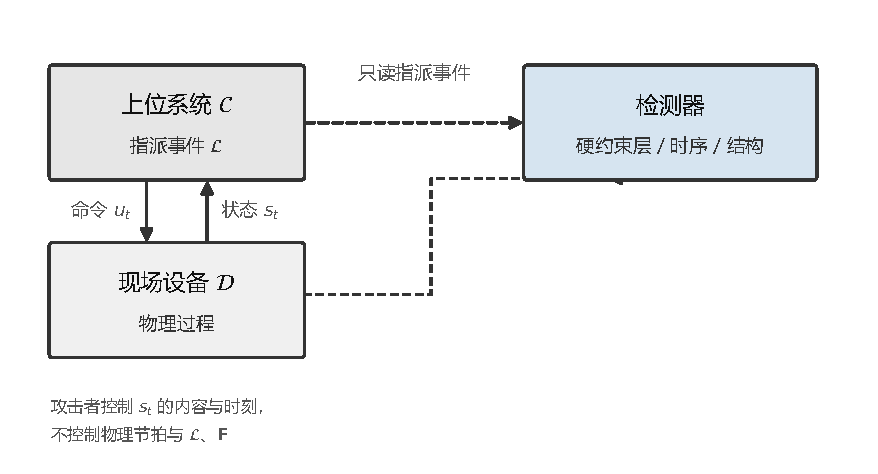
\includegraphics[width=0.92\linewidth]{figures/fig_system_CN.pdf}
\caption{命令/事件回环。检测器只读同一日志中的指派事件与参考模型可行性掩码，对上行事件作在线判决。}
\label{fig:system}
\Description{上位系统与现场资源构成指派下行、事件上行的回环，检测器只读指派事件并对上行事件作硬约束层、时序与结构三路判决。}
\end{figure}

\subsection{指派配对与可行性掩码}
\label{sec:ledger}

同一条事件日志记录下行指派，记为 $\mathcal{L}$。完成事件本应是某条指派的响应：若 $s_t$ 在对应 $(d,\mathrm{case})$ 上不存在前置指派，则构成一步即可判定的因果缺失。智能工厂将流程管理与现场事件流双向集成后，该配对关系可直接从日志中读取~\cite{seiger2022factory}。指派--完成属于因果检查，而非时长检验---指派到开始之间的排队时延主要由资源竞争决定，不宜纳入时序通道。

可行性由随产线发布的参考过程模型（本文为 {BPMN}）导出，记为掩码 $\mathbf F$。它含两类硬约束。\emph{一元能力集}：设备 $d$ 是否允许执行操作 $o$，不依赖前驱，覆盖全部消息。\emph{二元可达}：在同一 case、同一设备上，从已确认前驱 $o'$ 到 $o$ 是否被模型允许。二者均无法从运行日志中学习得到：日志只能给出历史上出现过的组合，无法区分``未曾观测''与``不允许''。同一份参考模型还可导出物料令牌等跨设备不变量，但在缺少工件级身份时，这类约束存在残余的良性违反，本文不将其纳入检测器。

\subsection{建模假设}
\label{sec:assumptions}

下列约定已散见于回环与威胁描述，此处集中写出，后文不再另立新假设。
第一，检测器只读上行事件与同一日志中的指派，不评测上位系统随后如何改派工。
第二，主实验日志为事件驱动上报；周期轮询只在方法中保留分支，不作跨域评测。
第三，攻击者按 {Dolev--Yao} 作用于上行链路，不能改写物理过程、设备固件或日志中已写入的指派。
第四，多资源协同伪造与物料令牌硬约束层均不在范围内：前者不予实现，也不报告结果；后者因缺少工件身份，仅作为局限讨论。

\subsection{攻击类型与通道覆盖}
\label{sec:coverage}

攻击者能力按 {Dolev--Yao} 模型~\cite{dolev1983yao}作用于上行链路：窃听、重放、注入、丢弃或延迟；可以知道状态机结构乃至转移频率。攻击者不能攻破上位系统或资源固件，不能改变物理世界，也不能改写日志中已写入的指派事件。目标是使事件记录与物理过程脱节。

表~\ref{tab:coverage}列出六类注入，表~\ref{tab:inject}给出可复现规则。生产检测器仅含三路：硬约束层 $\mathbf F$（含指派--完成）、结构通道与时序通道。主要检测对象是 {A2} 与 {A3}/{A5}；{A1} 作为重放对照，{A4}/{A6} 用于界定能力边界，不作为与先行工作对照的主要论据。多资源协同伪造（需同时对齐多路事件与指派）超出本文范围，不予实现与报告。

\begin{table}[!t]
\renewcommand{\arraystretch}{1.15}
\caption{六类事件注入与三路生产通道的单消息覆盖。括号内为同一批良性事件上的误报；{A2} 硬约束层的 $0.06$ 来自原地改写后、后继良性事件与伪造前驱的级联比对，其部署语义为``已检出攻击，但归因至后一条事件''，并非纯良性误报，故与第~\ref{sec:e1}~节的纯良性流误报分开报告。}
\label{tab:coverage}
\centering
\small
\begin{tabular}{llccc}
\toprule
编号 & 类型 & 硬约束层 $\mathbf F$ & 结构 & 时序 \\
\midrule
{A1} & 朴素重放 & $0.22\,(0.00)$ & $0.19\,(0.02)$ & $0.03\,(0.03)$ \\
{A2} & 物理不可行注入 & $0.98\,(0.06)$ & $0.29\,(0.03)$ & $0.00\,(0.02)$ \\
{A3} & 提前完成重放 & $0.00\,(0.00)$ & $0.02\,(0.01)$ & $0.43\,(0.02)$ \\
{A4} & 状态模仿（已知模型） & $0.03\,(0.00)$ & $0.02\,(0.03)$ & $0.00\,(0.02)$ \\
{A5} & 渐变漂移 & $0.00\,(0.00)$ & $0.01\,(0.01)$ & $0.48\,(0.03)$ \\
{A6} & 消息抑制 & $0.00\,(0.00)$ & $0.17\,(0.02)$ & $0.04\,(0.02)$ \\
\bottomrule
\end{tabular}
\end{table}

表~\ref{tab:coverage}的通道分工如下。{A2} 由一元能力集拒绝，时序通道对其不敏感。{A3}/{A5} 不改动标签，仅压缩或偏移停留时长，硬约束层与结构通道的检出接近于零，时序通道是唯一有实质提升的通道。{A1} 沿用历史时长，时序通道无增益，检出由硬约束层与结构通道承担。{A4} 按转移模型插入概率最大的下一步，三路通道的单消息检出均接近误报水平；{A6} 删除整条尚未开始的活动时，看门狗未被触发，结构通道仅在下游存在弱信号。指派--完成列为硬约束层的第三项，六类注入中没有专门破坏该配对的一类，故覆盖表未将其列为专属通道。因此，后文将可支撑的增益限定在 {A2} 与 {A3}/{A5}，而不在 {A4} 或指派配对。图~\ref{fig:coverage}将同一张表绘制为净提升热图，{A4} 所在行接近全白。

\begin{table}[!t]
\renewcommand{\arraystretch}{1.12}
\caption{六类注入的可复现规则。默认注入率 $20\%$，{A3}/{A5} 默认 $\rho=0.30$，三个随机种子；不改动 $\mathrm{case}$。{A4} 须提供结构模型，否则将退化为重复当前操作，从而低估攻击者能力。评测默认不整体前移同实例后继事件（$\texttt{shift\_downstream}=\mathrm{false}$）。}
\label{tab:inject}
\centering
\small
\begin{tabular}{lp{8.6cm}}
\toprule
编号 & 规则 \\
\midrule
{A1} & 将该资源的一条历史活动在当前完成时刻之后重发；时长沿用历史值，标签形成重复。 \\
{A2} & 原地将操作名改写为该资源能力集之外（若无则改为其他操作）的标签；后继良性事件可能与伪造前驱级联比对。 \\
{A3} & 原地将完成时刻提前，使停留时长变为 $(1-\rho)\tau$；默认不平移同实例的后续事件。 \\
{A4} & 已知模型：在当前完成之后插入转移概率最大的下一步，资源取日志中执行过该操作的设备，时长取该分组的中位数。 \\
{A5} & 在时间序上取一段连续活动，对各条施加同一 $\rho$ 的停留压缩（区别于 {A3} 的零散抽样）。 \\
{A6} & 整条删除尚未开始的活动；标注于同实例的后继事件上（可观测后果出现在下游）。 \\
\bottomrule
\end{tabular}
\end{table}

\begin{figure}[!t]
\centering
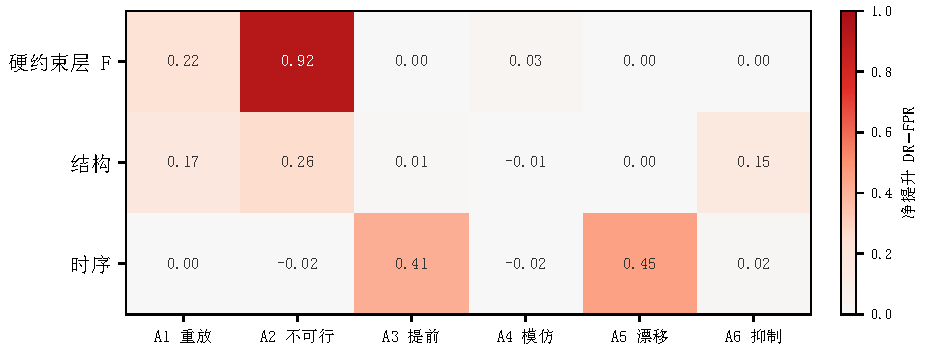
\includegraphics[width=0.98\linewidth]{figures/fig_coverage_CN.pdf}
\caption{三路生产通道相对良性误报的净提升（{DR}$-${FPR}）。{A2} 由硬约束层覆盖，{A3}/{A5} 仅时序通道有实质提升，{A4} 不存在专属通道。}
\label{fig:coverage}
\Description{三行六列热图：硬约束层、结构、时序对 A1 至 A6 的净检出提升，A2 硬约束层与 A3、A5 时序为深色高值，A4 接近零。}
\end{figure}

\subsection{检测问题}
\label{sec:detproblem}

\begin{problem}[离散事件注入检测]
\label{prob:detect}
给定仅含正常运行的历史日志、参考过程模型以及用户指定的误报预算 $\alpha$，对在线事件流逐条输出告警，使得纯良性流上的经验误报不超过 $\alpha$。主要检测对象是 {A2} 与 {A3}/{A5}；{A1}/{A4}/{A6} 一并报告，但不作为必须在预算内检出的承诺。检测器不得使用攻击标签调整阈值。安全目标是\emph{可检出，或伪造提前量有界}：未能在预算内检出的时长注入，其相对提前量受 $\rho^*(\alpha,\sigma)$ 限定（第~\ref{sec:bound}~节）。
\end{problem}

主要指标是同一 $\alpha$ 下、延迟预算内的净检出率（已扣除偶然告警基线，见第~\ref{sec:e1}~节），以消息数计的检测延迟（箱线图，仅含预算内检出），以及纯良性流上的实测 $\mathrm{ARL}_0$。计算约束为每条消息 $O(1)$。

% ============================================================
%  第 4 章：方法
% ============================================================
\section{检测方法}
\label{sec:framework}

\subsection{总体架构}
\label{sec:arch}

生产配置为三路并行，任一通道触发即告警。硬约束层良性违反率为零，\emph{不占用共形校准样本}；两路统计通道仍按三路并集分摊误报预算，各得 $\alpha/3$。这并非因为硬约束层存在误报，而是并行 {OR} 判决必须付出的代价：单通道方法独享全部 $\alpha$，而三路方法在仅有一路存在信号的攻击上，可用的误报预算只有单通道方法的三分之一。两路统计通道各自校准后由 {CUSUM} 累积。本文不设跨通道合成路径，也不将互锁统计通道纳入生产配置。

离线阶段仅使用正常日志与参考模型。由 {BPMN} 导出 $\mathbf F$；按设备与操作估计转移概率与停留时长；预留校准折，以共形预测确定两路统计通道的阈值，并在良性流上反向标定 {CUSUM} 门限，使目标平均误报间隔 $\mathrm{ARL}_0=1/\alpha$。在线阶段对每条消息执行常数次查表与对数运算，如图~\ref{fig:arch}。

\begin{figure}[!t]
\centering
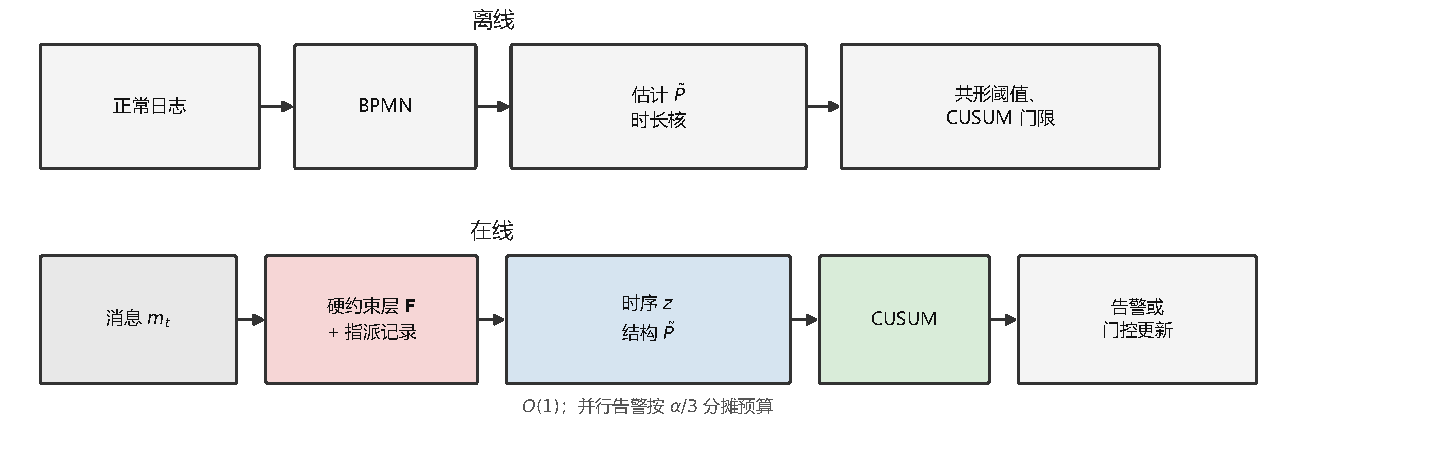
\includegraphics[width=0.98\linewidth]{figures/fig_arch_CN.pdf}
\caption{离线拟合与在线三路并行。硬约束层在统计通道之前，以免不可行样本污染校准；无互锁统计通道，无跨通道合成。}
\label{fig:arch}
\Description{离线阶段由日志与BPMN估计转移、时长核并校准阈值；在线阶段对每条消息依次做硬约束层否决、时序与结构打分及CUSUM累积。}
\end{figure}

硬约束层须置于最前：其判决代价为零、结果可解释，并可避免不可行样本进入后续校准。结构通道与时序通道并列而非串联，以便同时覆盖``标签错误''与``标签正确但时间错位''两类情形。序贯检验置于最后，因此两路统计通道必须输出分级分数而非布尔判决。算法~\ref{alg:detect}给出在线处理流程。

\begin{algorithm}[!t]
\caption{离散事件注入的在线检测}
\label{alg:detect}
\begin{algorithmic}[1]
\Require 事件 $m=(d,o,t)$；指派 $\mathcal{L}$；掩码 $\mathbf{F}$；核 $(\tilde P,\mu,\sigma)$；共形阈值与门限 $h$
\Ensure 告警或接受
\If{一元能力、二元可达或指派--完成任一违反}
    \State \textbf{return} 告警（硬约束层原因）
\EndIf
\State 计算时序残差 $z$ 与结构分数 $\tilde P_{o'\to o}$
\State 用冻结的共形校准器把两路分数映射为不符合度
\State 对两路分别更新 $S\leftarrow\max(0,\,S+s-c)$
\If{任一路 $S\ge h$}
    \State 复位该路；\textbf{return} 告警
\EndIf
\If{隔离窗口内无告警}
    \State 门控更新 $(\mu,\sigma,\tilde P)$ 并锚定状态
\EndIf
\State \textbf{return} 接受
\end{algorithmic}
\end{algorithm}

图~\ref{fig:alarm}逐条解析两个真实案例。{A2} 由一元能力集立即否决，并给出可读的告警原因；{A3} 的标签完全合法，其落在区间守卫内侧的负残差经 {CUSUM} 累积后越过门限。

\begin{figure}[!t]
\centering
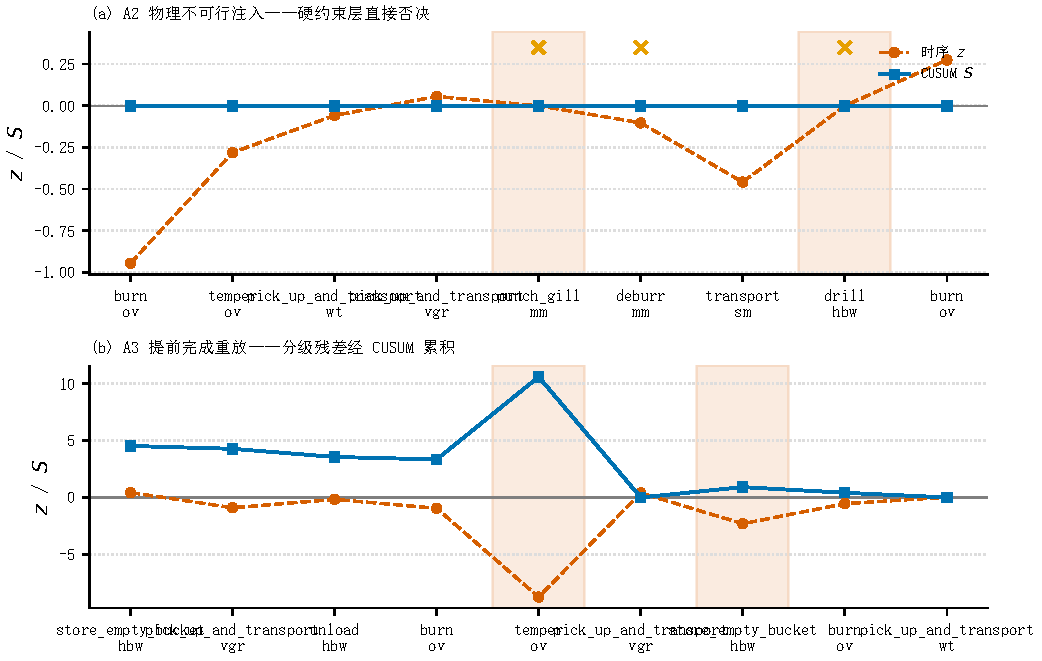
\includegraphics[width=0.98\linewidth]{figures/fig_alarm_CN.pdf}
\caption{{A2} 硬约束层否决与 {A3} 分级时序证据的逐条解析。阴影列为注入消息；叉号表示硬约束层触发。}
\label{fig:alarm}
\Description{上下两行为逐条解析：上行 A2 在注入处被硬约束层否决；下行 A3 的时序残差为负，CUSUM 随后越过门限。}
\end{figure}

\subsection{硬约束层可行性与指派--完成}
\label{sec:hard}

对消息 $(d,o,t)$，硬约束层依次检查三项，任一失败立即告警并给出原因。
\begin{enumerate}[leftmargin=1.4em,itemsep=2pt]
\item 一元：$(d,o)$ 是否属于参考模型的能力集。
\item 二元：若同一 $(d,\mathrm{case})$ 存在已确认前驱 $o'$，则 $(o'\to o)$ 是否被 $\mathbf F$ 允许。
\item 因果：该完成事件是否存在前置指派事件。
\end{enumerate}
掩码由随数据集发布的 {BPMN} 自动导出：一元能力集取自节点上绑定的设备类型（或资源角色），二元可达关系由同一工作流内的顺序结构与网关展开得到，无需手工编写转移表。一元检查覆盖全部消息，在正常数据上的违反率为零。时间序测试折中有 $20/508$（$3.9\%$）的良性活动属于训练折中未出现的 $(\text{设备},\text{操作})$ 组合，其比例远高于 $\alpha=0.01$，而参考模型对其中 $0$ 条作出拒绝。因此，训练折中未出现不能作为异常判据；指派--完成是同一硬约束层的第三项，覆盖表~\ref{tab:coverage}未为其单列攻击族。

\subsection{结构通道}
\label{sec:struct}

结构通道判定的是：当前活动在 case 级工作流序列上是否常见。链的粒度取 case 而非 $(d,\mathrm{case})$：在服务端点型产线上，设备级事件链大量长度为~$1$，转移概率缺乏区分度。通道状态取操作名，而非 $(\text{设备},\text{操作})$。后者看似可使结构通道识别``错误的设备执行了正确的操作''，但实测在三项指标上均为负收益：时间序划分下未出现的组合增多，经验误报升至名义值的约五倍；词表外状态触发弃权判决，{A2} 的结构检出由 $0.35$ 降为零；{A4} 无收益。``错误设备''属于一元能力硬约束，不应由统计通道对未出现的组合赋予过小的 $p$ 值---在时间序划分下，良性数据本身即会产生新组合。转移概率采用 {Dirichlet} 后验预测 $\tilde P$，以避免小样本导致的伪零，同时保留由 $\mathbf F$ 强制的真零。

输入共形校准器的是预测概率 $\tilde P_{o'\to o}$，而非随机化 $p$ 值。随机化的作用，是在分数直接与 $\alpha$ 比较时打散离散分布中大量取值相同所造成的并列；而输入校准器时应保留原始分数的次序，并列仅在阈值处打破一次。该通道对 {A4}/{A6} 这类改变事件数目的攻击较为敏感，但在三路均分误报预算后，其单路功效低于独享 $\alpha$ 的纯马尔可夫检测器---这是多通道方案的固有代价，见第~\ref{sec:e2}~节。

\subsection{半马尔可夫时序通道}
\label{sec:timing}

半马尔可夫核写作 $Q_{o'o}(\tau)=P_{o'o}F_{o'o}(\tau)$。停留时长按 $(\text{设备},\text{操作})$ 分组，取 $\log\tau\sim\mathcal{N}(\mu,\sigma^2)$。时序建模本身不是创新点；与计时自动机的差别在于 $F_{o'o}$ 为概率分布而非区间守卫，见第~\ref{sec:md}~节。生产配置未纳入路线协变量：在全局样本量加权口径下，条件化仅使 $\sigma$ 由 $0.236$ 降至 $0.228$，端到端无增益。

四种观测对应四个分支。
\begin{itemize}[leftmargin=1.4em,itemsep=2pt]
\item \textbf{状态跳变。} 标准化残差 $z=(\log\tau-\mu)/\sigma$，仅作左侧检验（停留时长过短即为提前上报）。提前上报对应有方向的备择假设；采用单侧检验的价值主要在于阈值稳定，而非功效成倍提升。
\item \textbf{同状态心跳。} 右删失生存函数 $-\log\bigl(1-F(\tau)\bigr)$，仅在停留时长过长时告警。
\item \textbf{超时无消息。} 采用同一生存函数，由看门狗在高分位触发。该分支可覆盖``活动已开始但完成事件被抑制''的情形，而无法覆盖``活动整条从未开始''的情形---后者需要活动间隔模型，本文不提供。
\item \textbf{周期轮询。} 区间删失 $\log\bigl[F(\tau+\Delta)-F(\tau)\bigr]$，以免量化误差污染似然。主实验为事件驱动日志，该分支不参与评测。
\end{itemize}
不符合度分数取 $z$ 本身，而不取参数化 $p$ 值。人工工位的 $\sigma$ 可接近~$2$，时序通道在此类分组上接近失效；整体检测能力由变异最大的工序决定。

\subsection{共形校准与序贯累积}
\label{sec:conformal}

两路统计通道在留出的正常样本上做分割共形预测~\cite{shafer2008conformal,angelopoulos2023conformal}，经验分位数在\emph{可交换}口径下给出 $\mathrm{FPR}\le\alpha/3$ 的阈值。该保证不依赖高斯或马尔可夫假设成立，但依赖校准集与部署数据可交换~\cite{barber2023exchangeability}。在随数据发布的 $16$ 个工作流之间两两计算转移集合的 {Jaccard} 相似度，中位数为 $0.324$，故新产品型号须重新校准或按型号分层。部署阶段只能按时间序划分，可交换性并不自动成立：名义 $\alpha=0.01$ 下，时序通道的经验误报由随机折的 $0.006$ 升至时间序的 $0.024$，结构通道由 $0.008$ 升至 $0.012$（表~\ref{tab:fprsplit}）。因此，贡献中所述的共形保证仅在随机折口径下成立；可部署口径见第~\ref{sec:boundary}~节。非交换性的影响主要体现在时序通道上。本日志的校准集规模为 $n_{\mathrm{cal}}=701$，可支撑的最低单消息 $\alpha$ 约为 $10^{-2}$；更低的误报预算由 {CUSUM} 的 $\mathrm{ARL}_0$ 承担。

不符合度分数必须在尾部保持单调次序。时序通道输入标准化残差 $z$，而非截断后的参数化 $p$ 值：当 $p$ 值在 $10^{-12}$ 处触及下限后，良性失配与 $30\%$ 的提前上报被压缩为同一取值，二者无法再区分，{A3} 的单消息检出由 $0.43$ 降至 $0.03$。结构通道同理输入 $\tilde P$，而非随机化概率积分变换。随机化仅用于直接与 $\alpha$ 比较的 $p$ 值；校准器上的并列情形仅在阈值处打破一次。

对各通道的不符合度分数做单侧 {CUSUM}~\cite{li2015quickest}
\begin{equation}
  S_t=\max\bigl(0,\,S_{t-1}+s_t-c\bigr),
  \label{eq:cusum}
\end{equation}
越过门限 $h$ 则告警并复位。$h$ 由良性流标定，目标 $\mathrm{ARL}_0=1/\alpha$。设计位移取 $1\sigma$。告警后必须复位，否则统计量将持续停留在门限之上，导致后续每条消息均触发告警。基线中凡输出分级分数的方法均采用同一累积规则，以免将增益误归因于 {CUSUM} 本身。

\subsection{门控更新与复杂度}
\label{sec:online}

正常消息用于锚定状态，并以指数滑动平均缓慢更新 $(\mu,\sigma)$ 与 $\tilde P$。更新必须门控：仅当该消息通过全部通道、且隔离窗口内无告警时，才允许进入基线。否则攻击者可通过持续的小幅提前上报，逐步将时长基线拉向伪造值。抗投毒相关数据来自在线回放诊断，不属于第~\ref{sec:e1}~节的主表结果，见第~\ref{sec:gate}~节。

单条消息的计算复杂度为 $O(1)$：常数次查表、对数运算与硬约束层判断，在热路径上与状态数、设备数无关。多设备可按链并行处理。第~\ref{sec:e8}~节给出常数因子。

% ============================================================
%  第 5 章：理论分析
% ============================================================
\section{理论分析}
\label{sec:theory}

\subsection{仅标签阈值族对标签自洽注入的不可能性}
\label{sec:ta}

考虑一类仅使用标签的检测器：由前驱 $i$ 得到预测分布 $\hat{\mathbf p}$，观测为 one-hot 向量 $\mathbf e_j$，以 $\delta(i,j)=\|\mathbf e_j-\hat{\mathbf p}\|_2$ 或任一严格随 $p_j$ 单调递减的变换与自适应阈值作比较。展开
\begin{equation}
  \delta(i,j)^2=1-2p_j+\|\hat{\mathbf p}\|^2
\end{equation}
由此可见，$\|\hat{\mathbf p}\|^2$ 对同一行的所有 $j$ 均为常数，$\delta$ 仅是 $p_j$ 的单调变换，几何结构不提供额外信息。因此 $\delta$ 是 $(i,j)$ 的确定性函数，与该消息为良性还是注入无关。在零误报约束下，``能够检出注入 $j$''当且仅当每一次良性的 $j$ 也触发告警，即 $\mathrm{DR}(j)>0\Rightarrow\mathrm{FPR}_i\ge p_j$。可标记集合恰为 $\{j:p_j=0\}$，即可行性掩码已经拒绝的转移；对标签自洽的注入，该检测族相对掩码的增量贡献恒为零。攻击者的最优规避目标为 $\arg\min_j\delta_j=\arg\max_j p_j$，而该转移恰好也是日志中最常见、伪造后最接近良性众数的下一步。

该结论不依赖具体的阈值系数，也不针对某一未发表的实现：凡判决仅为预测概率的一元函数的检测器，均属于该族。第~\ref{sec:e1}~节以一阶马尔可夫消融给出实证：在纯时序攻击 {A3}/{A5} 上，扣除偶然告警基线后的净检出为 $-0.01$ 与 $0.00$。

\subsection{分布型时长与时钟守卫}
\label{sec:md}

计时自动机对转移 $(o',o)$ 给出时钟守卫 $[\ell,u]$：$\tau\in[\ell,u]$ 则接受，否则拒绝~\cite{maier2011timed,lin2018tabor}。设正常停留时长的均值为 $\mu$。若攻击者取相对提前量 $\rho$，使 $(1-\rho)\mu\in[\ell,u]$，则该观测落在守卫之内，单步判决为正常。由于守卫为二值判断，同一方向上多次略偏快的停留不会被累积。

半马尔可夫通道输出的是分级残差 $z=(\log\tau-\mu)/\sigma$。提前上报使 $\mathbb{E}[z]=\log(1-\rho)/\sigma<0$。只要该期望低于 {CUSUM} 的参考值，累积统计量即以正漂移越过 $h$，即使每条观测的 $|z|$ 均小于单消息共形阈值。这并非停留时长建模本身的新颖性，而是\emph{证据形态}的差别：区间守卫将落在内侧的提前上报映射为零，分布型残差则将其映射为可加的增量。图~\ref{fig:guard}给出示意：全部观测落在守卫之内，二值通道不告警，{CUSUM} 仍越过门限。{A3} 正是这一差别所对应的典型情形---其标签完全合法，计时自动机予以接受，而序贯半马尔可夫仍可能检出。

\begin{figure}[!t]
\centering
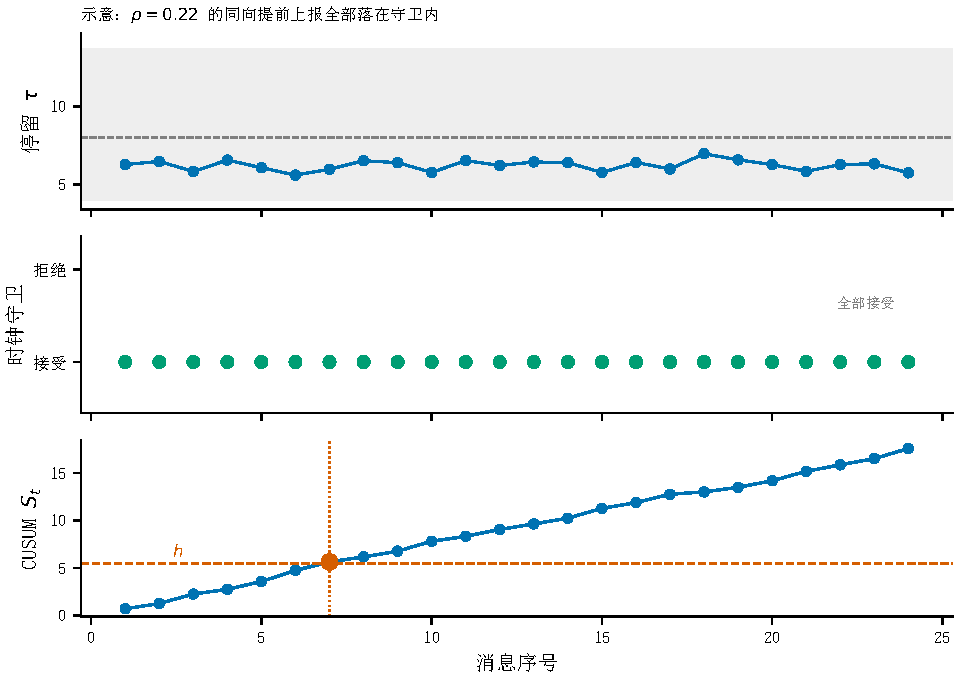
\includegraphics[width=0.95\linewidth]{figures/fig_guard_cusum_CN.pdf}
\caption{时钟守卫与分布型残差的差别（示意，非评测轨迹）。灰色带为区间守卫；同向提前上报全部被接受，{CUSUM} 仍累积越过 $h$。}
\label{fig:guard}
\Description{三行示意：停留时长均落在灰色守卫带内，时钟守卫全部接受，CUSUM 统计量随后越过门限。}
\end{figure}

\subsection{规避检测的相对提前量上界}
\label{sec:bound}

\begin{proposition}[规避检测的相对提前量上界]
\label{prop:rho}
设正常停留满足 $\log\tau\sim\mathcal{N}(\mu,\sigma^2)$，左侧水平为 $\alpha$，阈值为 $-z_{1-\alpha}$。攻击将观测时长缩为 $(1-\rho)\tau$。使攻击后残差均值恰好落在阈值上的相对提前量为
\begin{equation}
  \rho^*(\alpha,\sigma)=1-e^{-\sigma z_{1-\alpha}}.
  \label{eq:rho}
\end{equation}
$k$ 次独立重复下，均值标准差按 $1/\sqrt{k}$ 收缩，
\begin{equation}
  \rho^*_k(\alpha,\sigma)\approx 1-e^{-\sigma z_{1-\alpha}/\sqrt{k}}.
  \label{eq:rhok}
\end{equation}
\end{proposition}

\begin{proof}
对数域位移 $\Delta=\log(1-\rho)$，标准化后均值移动 $\Delta/\sigma$。令 $\Delta/\sigma=-z_{1-\alpha}$，解出 $\rho=1-e^{-\sigma z_{1-\alpha}}$。$k$ 次独立平均把 $\sigma$ 换成 $\sigma/\sqrt{k}$，即得式~\eqref{eq:rhok}。
\end{proof}

式~\eqref{eq:rhok}是重复注入条件下的收紧结果，本文实验仅验证单次注入的混合功效曲线，不将 $\sqrt{k}$ 的收缩写作已验证结论。式~\eqref{eq:rho}仅包含时序变异、误报预算与重复次数，不含系统矩阵。它是隐蔽攻击基本极限~\cite{liu2022limits}在离散事件场景下的实例：结论形式本身并不新颖，新的是其实例化对象为相对提前量，而非连续状态的偏差能量。对\emph{单一}高斯分布，均值恰落在阈值上所对应的单消息检出率约为 $1/2$。产线各工序的 $\sigma$ 高度异质，低变异分组在远小于全局 $\rho^*$ 的相对提前量下即可被检出，因而\emph{混合}功效曲线在 $\rho<\rho^*$ 时即可明显高于 $1/2$；第~\ref{sec:e4}~节验证的是该混合曲线与实测结果的吻合程度，而非``超过 $\rho^*$ 之后才达到半数''。图~\ref{fig:sigma}给出 $\rho^*(\sigma)$ 曲线：全局 $\sigma=0.236$ 对应 $42.2\%$；人工工位的 $\sigma$ 接近 $2$ 时该上界失效，产线整体的可检测性由最薄弱环节决定。

\begin{figure}[!t]
\centering
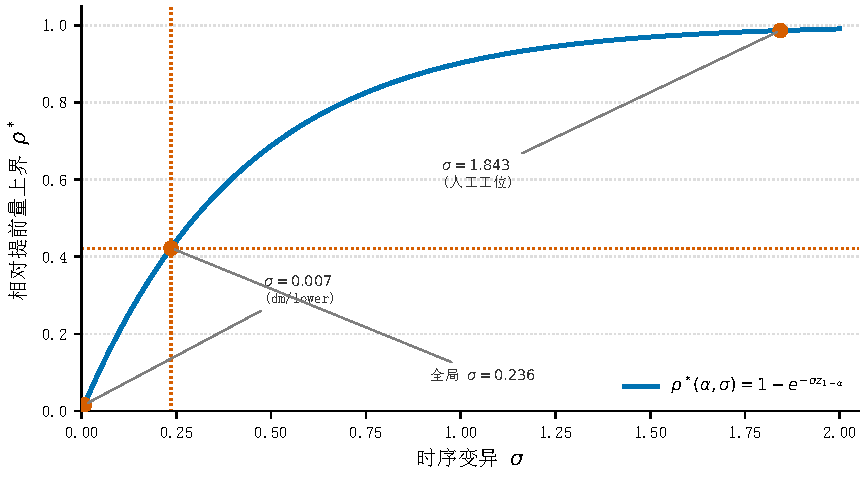
\includegraphics[width=0.82\linewidth]{figures/fig_sigma_CN.pdf}
\caption{$\alpha=0.01$ 单侧下 $\rho^*$ 随 $\sigma$ 的变化。标注点为低变异工序、全局加权 $\sigma$ 与人工工位。}
\label{fig:sigma}
\Description{相对提前量上界随时序变异增大并趋近于一，全局 sigma 为 0.236 时上界约百分之四十二。}
\end{figure}

% ============================================================
%  第 6 章：实验
% ============================================================
\section{实验与结果分析}
\label{sec:experiments}

\subsection{实验设置}
\label{sec:setup}

主数据采用 {University of Trier} 教学工厂发布的 {Fischertechnik} 智能工厂 {IoT} 事件日志~\cite{malburg2022trier}。选用理由在于：它是目前少有的、同时提供 {BPMN} 参考模型与指派--执行--完成生命周期的公开活动日志，而非因其规模具有代表性。{HAI} 等 1~Hz 过程量标签无法实例化指派与工序活动~\cite{shin2020hai}，工业控制系统测试床与公开数据集的综述亦以过程量与网络流量为主~\cite{conti2021testbeds,dobler2025datasets}，故本文不报告跨域结果。日志内部的多样性用于压力测试，不作为第二份外部数据：随数据发布的 {BPMN} 共 $16$ 个；官方含错版本（NTP 漂移、重复、缺失）用于误报压力测试；时间序测试折包含训练折中未出现的五个工作流。产线上十余台资源均为被调用的服务端点，按资源切分的状态链多数长度为~$1$，因此结构通道须采用 case 级工作流链。一元能力集取自节点绑定的设备类型，二元可达关系取同一工作流内顺序结构与网关的传递闭包，由此自动得到 $\mathbf F$。清洗后全日志共 $3{,}062$ 条活动。

公开活动日志不含注入标注~\cite{conti2021testbeds,dobler2025datasets}。本文将 {Dolev--Yao} 模型中的重放、注入与丢弃映射到本日志的字段上，规则见表~\ref{tab:inject}，注入器随代码发布。注入在测试折上实施，主表注入率为 $20\%$，并扫描 $5\%/10\%/20\%/40\%$；相对提前量默认 $\rho=0.30$，使用三个随机种子。{A4} 须提供结构模型。数据划分按时间序进行：拟合、校准与测试三部分互不重叠；测试折含良性事件 $508$ 条，E1 选择折 $603$ 条。时序通道的共形校准另用按组分层的校准折，$n_{\mathrm{cal}}=701$。检测延迟按注入实例存档，箱线图仅含预算内检出的实例。生产配置冻结为硬约束层、时序与结构三路。

三项主基线均按原文的结构约束复现，而非使用官方代码：Maier/{BUTLA} 与 {TABOR} 未随文发布可对接本日志模式的实现，{HSMM} 属于模型类而非工业检测器。表~\ref{tab:repro}列出复现中的保留项与近似项。凡输出分级分数的方法均采用同一套 {CUSUM}（延迟预算 $10$ 条，告警后复位），并在同一良性参照流上将经验误报对齐至 $\alpha$。符合度代理（违反 $\mathbf F$ 即告警）与硬约束层重合，故不在主表中单列；第~\ref{sec:e2}~节中去掉时序通道后的配置即为该对照。仅标签的一阶马尔可夫似然属于消融配置，而非独立的先行方法。阈值在同一批 case 的未注入版本上确定，不使用受攻击流内部的良性事件。

\begin{table}[!t]
\renewcommand{\arraystretch}{1.12}
\caption{主基线的复现协议。对照的是原文结构约束，不是官方二进制。}
\label{tab:repro}
\centering
\small
\begin{tabular}{lp{3.4cm}p{4.4cm}}
\toprule
方法 & 保留 & 本日志上的近似 \\
\midrule
{B3} {BUTLA} 式~\cite{maier2011timed}
  & 按组件各学一台自动机；无跨组件检查；时长为偏离容差
  & 组件取为资源；容差改为同 $\alpha$ 下的经验分位，以免将误报差异误计为方法差异 \\
{B4} {TABOR} 式~\cite{lin2018tabor}
  & 站内依赖；显式不使用命令数据
  & 站取为资源；站内采用 $P(o)\prod P(v\mid o)$（该近似倾向于高估原文结构的能力） \\
{B5} {HSMM}~\cite{tan2008hsmm}
  & 显式时长的半马尔可夫模型
  & 观测为操作与 $\log\tau$；$K\in\{2,3,4,6\}$ 由留出似然选定为 $6$ \\
\bottomrule
\end{tabular}
\end{table}

在延迟预算内采用``窗口中出现任一告警即判为检出''的口径时，即使检测器不具备任何真实检测能力，窗口内的随机误报也会带来一定的检出率。该偶然告警基线为 $1-(1-\mathrm{FPR})^{B+1}$（$B=10$）。表中主结果均已扣除该基线；未扣除的数值不单独引用。逐消息检出率受参照流长度限制，在本规模下不作为主结果。

\subsection{与计时自动机及半马尔可夫的对照}
\label{sec:e1}

表~\ref{tab:e1}给出 $\alpha=0.01$ 下的净检出率。本方法的均值为 $0.48$，{B3}/{B4}/{B5} 分别为 $0.17/0.21/0.11$。本文不主张全面优于既有方法，而将结论限定为以下三点。第一，{A3}/{A5} 属于纯时序攻击，标签未发生改动；仅标签消融在扣除偶然告警基线后为 $-0.01$ 与 $0.00$，即其分数流与良性流逐条相同。证据最明确的一项是 {A5}：本文为 $0.87$，仅标签消融为 $0.00$。在 {A3} 上，本文为 $0.18{\pm}0.01$，{B3}/{B4} 为 $0.10{\pm}0.03$，相差约 $8$ 个百分点且区间不重叠---其机理在于检出非零且可累积，本文不宣称显著领先。在 {A5} 上，计时自动机同样可以捕捉累积式漂移（$0.59/0.48$），但仍低于按 $(\text{设备},\text{操作})$ 作左尾检验的分布型通道。{B5} 在 {A3} 上仅为 $0.06$，说明增益并非全部来自``半马尔可夫模型相对区间守卫''的模型类差异：其时长核绑定在隐状态上，标签未改的提前上报被吸收为一次略短的停留。第二，在 {A1}/{A2} 上本方法为 $0.55/0.95$，高于三条主基线；{A2} 由一元能力集覆盖，{B4} 的站内依赖无法替代参考模型。时间序测试折中 $20/508$（$3.9\%$）的未出现组合已被参考模型全部放行，见第~\ref{sec:hard}~节。第三，在 {A4}/{A6} 上本方法为 $0.17/0.14$，低于仅标签消融的 $0.23/0.28$---三路均分使结构通道仅获得 $\alpha/3$，而这两类攻击主要改变事件数目。这是多通道方法的预算代价，而非通道设计失效。需要说明的是，表~\ref{tab:coverage}是单通道、单消息、未扣除偶然告警基线的覆盖诊断，表~\ref{tab:e1}则是三路并行、延迟预算 $10$ 条、已扣除偶然告警基线的端到端净检出。因此 {A3} 的时序单消息检出 $0.43$ 与表~\ref{tab:e1}中的 $0.18$ 并不矛盾：后者将误报预算摊至 $\alpha/3$，并扣除了窗口的偶然告警基线。

\begin{table}[!t]
\renewcommand{\arraystretch}{1.15}
\caption{$\alpha=0.01$、延迟预算 $10$ 条、已扣除偶然告警基线的净检出率。三个随机种子的均值$\pm$总体标准差。仅标签为马尔可夫消融。序贯误报（名义 $0.01$）依次为 $0.006$、$0.006$、$0.008$、$0.004$（仅标签 $0.008$）。}
\label{tab:e1}
\centering
\scriptsize
\begin{tabular}{lccccc}
\toprule
攻击 & {B3} {BUTLA} & {B4} {TABOR} 式 & {B5} {HSMM} & 仅标签 & 本文 \\
\midrule
{A1} 朴素重放 & $0.04{\pm}0.01$ & $0.04{\pm}0.01$ & $-0.01{\pm}0.03$ & $0.48{\pm}0.04$ & $0.55{\pm}0.04$ \\
{A2} 不可行注入 & $0.37{\pm}0.05$ & $0.67{\pm}0.03$ & $0.31{\pm}0.04$ & $0.77{\pm}0.04$ & $0.95{\pm}0.01$ \\
{A3} 提前完成重放 & $0.10{\pm}0.03$ & $0.10{\pm}0.04$ & $0.06{\pm}0.04$ & $-0.01{\pm}0.02$ & $0.18{\pm}0.01$ \\
{A4} 状态模仿 & $-0.04{\pm}0.01$ & $-0.01{\pm}0.01$ & $0.02{\pm}0.01$ & $0.23{\pm}0.04$ & $0.17{\pm}0.03$ \\
{A5} 渐变漂移 & $0.59{\pm}0.09$ & $0.48{\pm}0.07$ & $0.25{\pm}0.08$ & $0.00{\pm}0.12$ & $0.87{\pm}0.06$ \\
{A6} 消息抑制 & $-0.05{\pm}0.01$ & $-0.01{\pm}0.03$ & $0.05{\pm}0.02$ & $0.28{\pm}0.08$ & $0.14{\pm}0.05$ \\
\midrule
均值 & $0.17$ & $0.21$ & $0.11$ & $0.29$ & $0.48$ \\
\bottomrule
\end{tabular}
\end{table}

图~\ref{fig:e1}将表~\ref{tab:e1}绘制为柱状对照。仅标签消融在 {A3}/{A5} 上贴近零线，反映去掉时间维度后形成的结构性盲区；本文在 {A4}/{A6} 上低于该消融，与三路均分预算的预期一致，本文不据此改写为全面优于。图~\ref{fig:e1delay}为同一评测的检测延迟箱线图：仅统计延迟预算内检出的注入，未检出实例不计入分位数。表~\ref{tab:arl0}为纯良性流上实测的平均误报间隔，与攻击流中的序贯误报分开统计；目标 $\mathrm{ARL}_0=1/\alpha=100$，本文的结果更为保守（中位 $218$），与序贯误报 $0.004$ 一致。图~\ref{fig:e1rate}将注入率从 $5\%$ 扫描至 $40\%$：{A2}/{A5} 的优势不随注入密度升高而衰减，{A3} 的检出保持非零，{A4}/{A6} 仍低于仅标签消融。

\begin{figure}[!t]
\centering
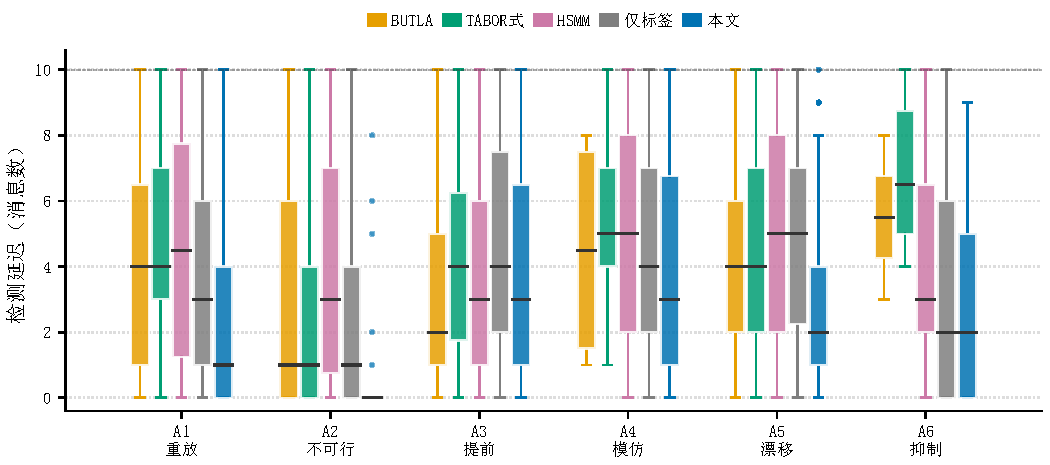
\includegraphics[width=0.98\linewidth]{figures/fig_e1_delay_CN.pdf}
\caption{$\alpha=0.01$、延迟预算 $10$ 条下，各方法在六类攻击上的检测延迟（消息数）。箱线仅含预算内检出；未检出见净检出率。}
\label{fig:e1delay}
\Description{六类攻击上 BUTLA、TABOR 式、HSMM、仅标签与本文的分组箱线图，纵轴为检测延迟消息数。}
\end{figure}

\begin{figure}[!t]
\centering
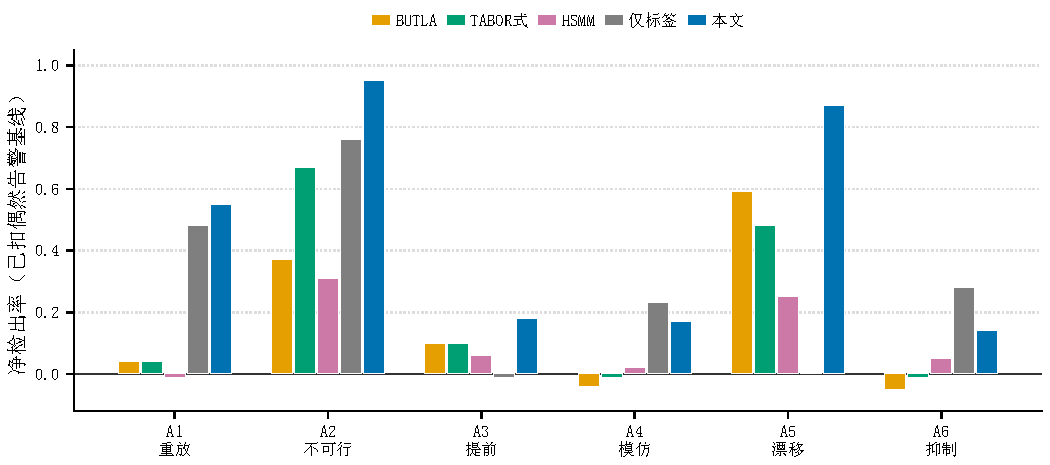
\includegraphics[width=0.98\linewidth]{figures/fig_e1_dr_CN.pdf}
\caption{$\alpha=0.01$、延迟预算 $10$ 条、已扣除偶然告警基线的净检出率。仅标签为马尔可夫消融，而非独立的先行方法。}
\label{fig:e1}
\Description{六类攻击上 BUTLA、TABOR 式、HSMM、仅标签与本文的分组柱状图，本文在 A2 与 A5 最高，仅标签在 A3 与 A5 为零。}
\end{figure}

\begin{table}[!t]
\renewcommand{\arraystretch}{1.12}
\caption{纯良性流上的实测 $\mathrm{ARL}_0$（目标 $100$）。中位与均值按告警间隔统计；告警次数为三个随机种子的合计。}
\label{tab:arl0}
\centering
\small
\begin{tabular}{lccc}
\toprule
方法 & 中位间隔 & 均值间隔 & 告警次数 \\
\midrule
{B3} {BUTLA} & $21$ & $152$ & $54$ \\
{B4} {TABOR} 式 & $59$ & $158$ & $54$ \\
{B5} {HSMM} & $119$ & $115$ & $72$ \\
仅标签 & $56$ & $83$ & $72$ \\
本文 & $218$ & $218$ & $36$ \\
\bottomrule
\end{tabular}
\end{table}

\begin{figure}[!t]
\centering
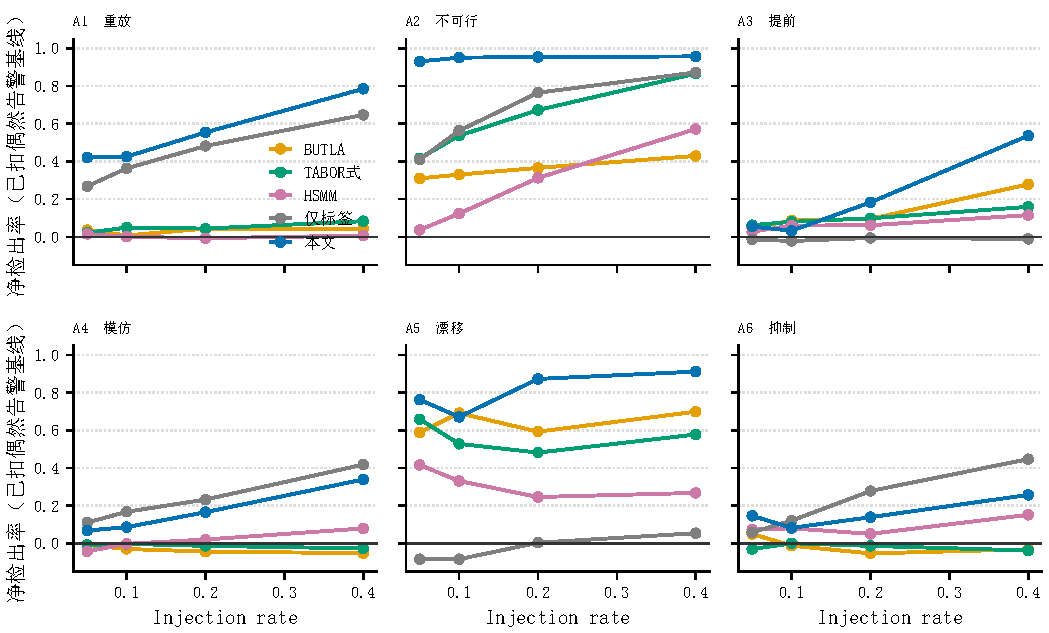
\includegraphics[width=0.98\linewidth]{figures/fig_e1_rate_CN.pdf}
\caption{净检出率随注入率（$5\%$--$40\%$）的变化。按攻击族分设子图，可据此判断结论是否随攻击密度升高而失效。}
\label{fig:e1rate}
\Description{六个攻击族子图，横轴注入率，纵轴净检出率，五条方法曲线。}
\end{figure}

{B4} 与 {B3} 在多数攻击族上表现接近：站内依赖在本日志上信息量较低，且其对``该设备从未执行过此操作''所赋予的极端分数，在良性测试折中即已出现（第~\ref{sec:hard}~节所述 $3.9\%$ 的未出现组合）。参考模型对这 $20$ 条中的 $0$ 条作出拒绝。{B5} 的 {EM} 似然单调收敛，时长核非退化，可作为与``时序加结构''直接对照的基线；其均值为 $0.11$，说明将状态处理为隐变量并不能自动获得可行性掩码。按校准折确定阈值后，测试折上的误报为：{B3}/{B4} 为名义值的 $3.7$ 倍，{B5} 为 $1.0$ 倍。因此，共形方法的对照意义并不在于``仅本文能够控制误报''，而在于该控制不依赖模型假设成立。在 $\alpha=0.05$ 下各项排序不变，{A4}/{A6} 的劣势并非分辨率造成的假象。

\subsection{消融}
\label{sec:e2}

消融实验在 $\alpha=0.05$、\emph{每路误报预算固定}的设置下进行，以避免``去掉一路通道等同于为其余通道增加预算''的混淆。完整配置在六个攻击族上的均值为 $0.41$。去掉时序通道后均值下降 $0.11$，且 {A3}/{A5} 精确归零（$0.27\to 0.01$，$0.70\to -0.02$）。去掉时序通道后的配置即为参考模型符合度代理（违反 $\mathbf F$ 即告警）：其可覆盖 {A2}，对纯时长攻击的检出为零。这与表~\ref{tab:e1}中仅标签消融在相同两项上的零检出，是同一现象的两项独立证据。去掉硬约束层后均值下降 $0.07$，降幅集中在 {A2} 与 {A1}。去掉结构通道后均值下降 $0.04$，降幅集中在 {A4} 与 {A6}。图~\ref{fig:e2}给出按攻击族的对照与均值变化。

\begin{figure}[!t]
\centering
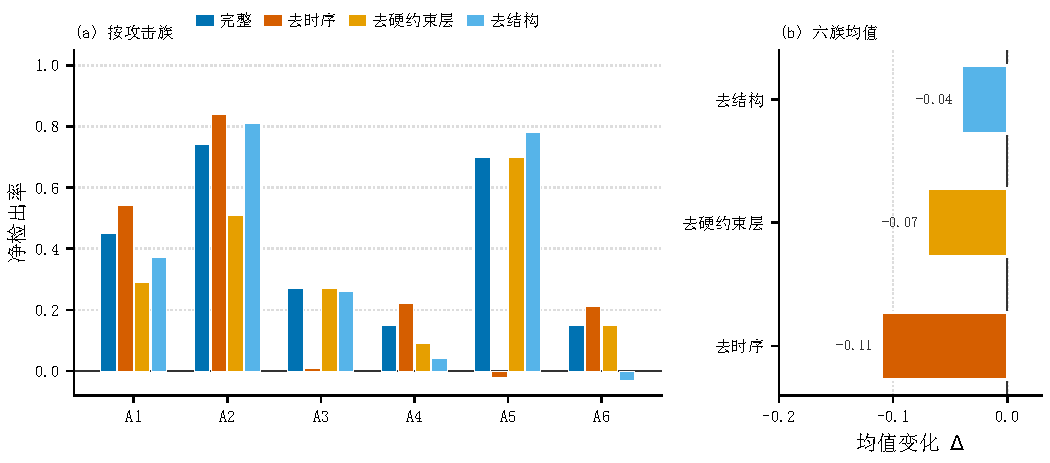
\includegraphics[width=0.98\linewidth]{figures/fig_e2_ablation_CN.pdf}
\caption{生产三路的消融（每路误报预算固定，$\alpha=0.05$）。去掉时序后 {A3}/{A5} 归零；硬约束层与结构的贡献分别集中在 {A2}/{A1} 与 {A4}/{A6}。}
\label{fig:e2}
\Description{左图为完整、去时序、去硬约束层、去结构在六类攻击上的柱状对照；右图为均值下降 0.11、0.07、0.04。}
\end{figure}

共形校准在检出率口径上的增益接近于零（$-0.01$），因为其作用在于对齐误报水平；相应证据体现在误报一侧：采用参数化阈值会使经验误报接近翻倍。物料令牌不变量与跨通道合成路径曾作为候选统计通道，但其在良性违反率上限与端到端消融两方面的净贡献均为非正，故不纳入生产配置，也不占用 $\alpha$ 预算。

\subsection{相对提前量与理论界}
\label{sec:e4}

在真实停留时长上施加注入 $\tau\mapsto(1-\rho)\tau$。命题~\ref{prop:rho}中的 $\rho^*$ 使用全局拟合折的 $\sigma=0.236$（不采用协变量口径）；$\alpha=0.01$ 单侧时 $\rho^*=42.2\%$。表~\ref{tab:e4}与图~\ref{fig:e4}的理论列为按工序分组后的混合预测，而不是将全局 $\sigma$ 代入单一高斯分布后、在 $\rho^*$ 处应等于 $1/2$ 的那一点：$\rho=0.30<\rho^*$ 时实测单消息检出为 $0.45$，$\rho=0.40\approx\rho^*$ 时为 $0.71$。全区间的平均绝对偏差约为 $0.03$。{CUSUM} 可将弱信号转化为可用的检测能力：$\rho=0.15$ 时单消息检出为 $0.20$，累积后升至 $0.87$，中位延迟为 $10$ 条消息；$\rho=0.30$ 时中位延迟为 $4$ 条，见图~\ref{fig:delay}。检出率在约 $0.96$ 处饱和，未检出部分来自 $\sigma$ 极大的分组，与``最薄弱环节''的表述一致。

\begin{table}[!t]
\renewcommand{\arraystretch}{1.12}
\caption{$\alpha=0.01$ 单侧下相对提前量扫描。位移 $\Delta=\log(1-\rho)$；理论列为按工序混合后的预测，不是全局 $\sigma$ 下单一高斯在 $\rho^*$ 处的 $1/2$ 点。}
\label{tab:e4}
\centering
\small
\begin{tabular}{ccccc}
\toprule
$\rho$ & $\lvert\Delta\rvert$ & $\lvert\Delta\rvert/\bar\sigma$ & 实测 {DR} & 理论 \\
\midrule
$0.05$ & $0.051$ & $0.21$ & $0.060$ & $0.051$ \\
$0.10$ & $0.105$ & $0.44$ & $0.105$ & $0.127$ \\
$0.15$ & $0.163$ & $0.68$ & $0.199$ & $0.226$ \\
$0.20$ & $0.223$ & $0.93$ & $0.288$ & $0.317$ \\
$0.30$ & $0.357$ & $1.49$ & $0.452$ & $0.497$ \\
$0.40$ & $0.511$ & $2.14$ & $0.712$ & $0.701$ \\
$0.50$ & $0.693$ & $2.90$ & $0.874$ & $0.851$ \\
\bottomrule
\end{tabular}
\end{table}

\begin{figure}[!t]
\centering
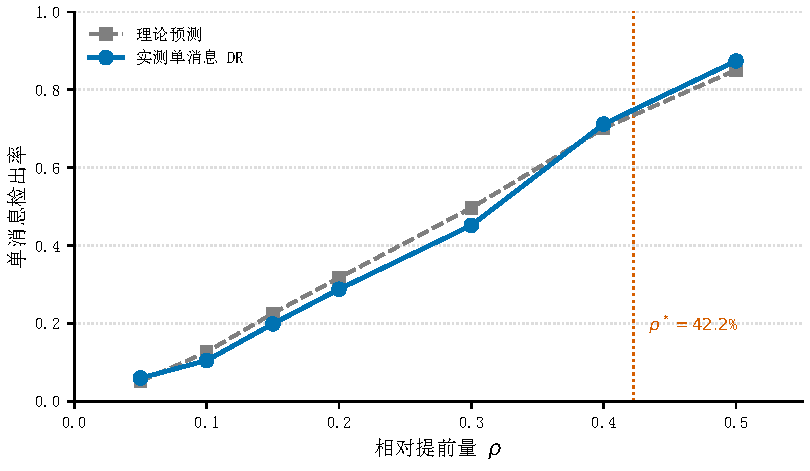
\includegraphics[width=0.82\linewidth]{figures/fig_e4_rho_CN.pdf}
\caption{单消息检出率随相对提前量的变化。理论列为分组混合预测；竖线为全局 $\sigma=0.236$ 下的 $\rho^*=42.2\%$。}
\label{fig:e4}
\Description{实测单消息检出率与按工序混合的理论预测随相对提前量上升；竖线标出全局 sigma 下的 rho 星，该处混合功效已明显高于二分之一。}
\end{figure}

\begin{figure}[!t]
\centering
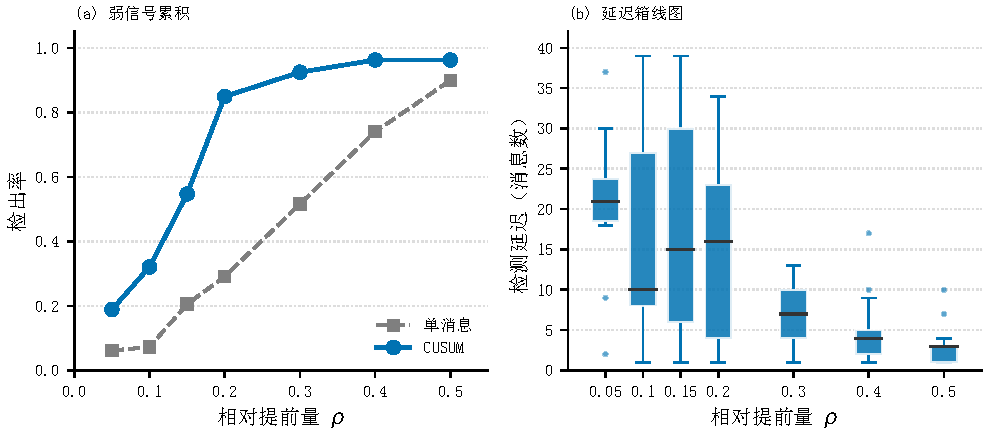
\includegraphics[width=0.98\linewidth]{figures/fig_delay_CN.pdf}
\caption{{CUSUM} 相对单消息阈值的功效，以及检测延迟箱线图。箱线只含预算内检出的注入；未检出为删失，见主表净检出率。}
\label{fig:delay}
\Description{左图 CUSUM 检出率在小相对提前量下明显高于单消息；右图中位延迟随相对提前量下降。}
\end{figure}

\subsection{部署口径与适用边界}
\label{sec:boundary}
\label{sec:e5}
\label{sec:robust}
\label{sec:gate}
\label{sec:e6}
\label{sec:e8}

主结果限于第~\ref{sec:e1}--\ref{sec:e4}~节。本节仅给出部署前必须声明的四组数据，其权重不与主表等同。

共形保证依赖可交换性假设。由表~\ref{tab:fprsplit}可见：随机折下的经验误报贴近名义值；时间序划分下，时序通道在 $\alpha=0.01$ 时升至 $0.024$，结构通道升至 $0.012$。该数值与第~\ref{sec:e1}~节的序贯误报 $0.004$ 不属于同一口径。实际部署不具备随机划分的条件。表~\ref{tab:shift}汇总了日志内部的压力测试：官方含错版本的时序误报为 $0.112$（源自数据采集缺陷的良性时序异常，并非攻击）；未出现工作流上的时序误报为 $0.067$，两种情形下硬约束层均为 $0$。产品切换属于分布漂移，时序通道须按型号重新校准，硬约束层则无此必要。将拟合折的 $\sigma$ 人为加倍后，$\rho=0.30$ 时的单消息/{CUSUM} 检出由 $0.52/0.94$ 降至 $0.22/0.45$；$\sigma\approx0.96$ 时单消息检出仅剩 $0.05$。适用边界由变异最大的工序划定。

门控属于架构约束，不计入主表：在持续 $200$ 条、$\rho=0.30$ 的提前上报下，关闭门控会将 $26.4\%$ 的伪造提前量引入基线（$200/200$ 次更新全部生效），启用门控后降至 $1.4\%$（$2/200$）。单核逐事件处理时延的中位数为 $73\,\mu\mathrm{s}$（$p_{95}=109$，$n=1{,}524$）；复制资源名以扩大规模后，中位时延不随规模上升。本文未在专用控制器上实测。

表~\ref{tab:e6}用于演示时长核必须按场景重新标定的机理，而非第二份外部数据：将短行程场景的时长核迁移至长行程场景后，{A3} 检出由 $0.56$ 降至 $0.06$；反向迁移则使时序误报达到 $0.493$。三种设置下硬约束层均为 $0$，原因是 $\mathbf F$ 相同。

\begin{table}[!t]
\renewcommand{\arraystretch}{1.12}
\caption{逐通道共形经验误报（五种子均值$\pm$标准差）。}
\label{tab:fprsplit}
\centering
\small
\begin{tabular}{lcccc}
\toprule
通道 & \multicolumn{2}{c}{随机折} & \multicolumn{2}{c}{时间序} \\
\cmidrule(lr){2-3}\cmidrule(lr){4-5}
 & $\alpha{=}0.05$ & $\alpha{=}0.01$ & $\alpha{=}0.05$ & $\alpha{=}0.01$ \\
\midrule
时序 & $0.051{\pm}0.007$ & $0.006{\pm}0.005$ & $0.098{\pm}0.001$ & $0.024{\pm}0.001$ \\
结构 & $0.048{\pm}0.013$ & $0.008{\pm}0.006$ & $0.064{\pm}0.003$ & $0.012{\pm}0.001$ \\
\bottomrule
\end{tabular}
\end{table}

\begin{table}[!t]
\renewcommand{\arraystretch}{1.12}
\caption{同一份 {Trier} 日志内部的压力测试（$\alpha=0.01$，不注入）。含错版本由原作者发布；未出现工作流由时间序测试折切分得到。}
\label{tab:shift}
\label{tab:cprime}
\label{tab:e9}
\centering
\small
\begin{tabular}{lcccc}
\toprule
场景 & $n$ & 硬约束层 & 时序 & 结构 \\
\midrule
清洗时间序测试折 & $508$ & $0.000$ & $0.024$ & $0.012$ \\
官方含错全日志 & $2{,}778$ & $0.003$ & $0.112$ & $0.011$ \\
已出现工作流 & $329$ & $0.000$ & $0.000$ & $0.012$ \\
未出现工作流 & $179$ & $0.000$ & $0.067$ & $0.006$ \\
\bottomrule
\end{tabular}
\end{table}

\begin{table}[!t]
\renewcommand{\arraystretch}{1.12}
\caption{时长核按场景重新标定（$\alpha=0.01$，$\rho=0.30$）。{A3} 为时序通道的单消息检出；该结果不作为外部效度的主要证据。}
\label{tab:e6}
\centering
\small
\begin{tabular}{lcccc}
\toprule
设置 & 硬约束层 & 时序 & 结构 & {A3} \\
\midrule
{A} 本场景 & $0.000$ & $0.000$ & $0.014$ & $0.462$ \\
{B} 本场景 & $0.000$ & $0.000$ & $0.011$ & $0.556$ \\
{C} 本场景 & $0.000$ & $0.000$ & $0.014$ & $0.308$ \\
{A}$\to${B} & $0.000$ & $0.000$ & $0.000$ & $0.056$ \\
{A}$\to${C} & $0.000$ & $0.101$ & $0.000$ & $0.385$ \\
{B}$\to${A} & $0.000$ & $0.493$ & $0.000$ & $0.692$ \\
\bottomrule
\end{tabular}
\end{table}

% ============================================================
%  第 7 章：结论
% ============================================================
\section{结论}
\label{sec:conclusion}

\subsection{结论与贡献}
\label{sec:contributions}

本文将离散工业事件流上的注入检测表述为一个独立问题：检测对象是带生命周期的活动事件（例如调度系统指派设备执行一项作业后，日志中的指派--开始--完成记录），而非连续控制或报文会话，也不评测调度器随后如何重新派工。仅依赖标签预测与自适应阈值的检测族，在零误报约束下对标签自洽的注入不提供超出可行性掩码的增量。在方法层面，硬约束层的主要证据是参考模型可行性掩码；指派--完成是同一硬约束层的第三项，六类注入未为其单列攻击族。时序通道按 $(\text{资源},\text{操作})$ 分组作左尾检验，与结构通道在可交换口径下完成共形校准后并行累积；部署阶段报告时间序经验误报率。相对于分解式计时自动机与站内依赖模型，可支撑的差别有两点：分布型时长使落在守卫内侧的提前上报可被累积；可行性无法从日志中学习得到。若将符合度用作检测器、以违反掩码作为规则，其判决与硬约束层重合，可覆盖 {A2}，而对 {A3}/{A5} 的检出为零。主表中证据最明确的两项是 {A5} 相对仅标签检测族的结构性非零检出，以及 {A2} 由掩码覆盖；{A3} 的检出保持非零，但增益小于渐变漂移。规避检测的相对提前量存在上界 $\rho^*(\alpha,\sigma)$，实验验证的是单次注入下的混合功效曲线。

\subsection{局限}
\label{sec:limitations}

\textbf{(1) 状态模仿与整段活动抑制缺少专属检测通道。}
二者在生产配置下均无专属通道，其在 {A4}/{A6} 上的检出低于仅标签检测器，原因是三路通道分摊误报预算后，结构通道可用的预算不足。

\textbf{(2) 物料流不变量在缺少工件身份时只能作为软约束层。}
训练折上的良性违反率为 $q=0.0054$，部署流中升至 $0.047$（漂移约九倍），$\alpha=0.01$ 下单消息检出的上限仅为 $0.21$。要使该通道可用，部署阶段的 $q$ 须降至 $\alpha$ 量级（约 $1\%$）；基于跨 case 的近似身份仅能降至 $2.3\%$，其余部分需依靠 {NFC}/{RFID} 工件标识。近似身份方案已经过验证，端到端表现与原口径持平，故令牌约束未被纳入现行通道。

\textbf{(3) 多资源协同伪造超出本文声明的范围。}
该情形未予实现，亦不报告相关结果。

\textbf{(4) 主评测仅使用一份公开日志、合成注入与复现基线。}
主评测仅有一份同时具备 {BPMN} 与活动生命周期的公开日志，攻击由可复现的注入器合成，基线按原文结构约束复现而非使用官方代码。日志内部通过 $16$ 个工作流、官方含错版本与未出现工作流进行切分，用于压力测试，不作为第二份外部数据。共形保证仅在可交换口径下成立：时间序划分下时序误报升至 $0.024$，未出现工作流上为 $0.067$，含错时间戳条件下为 $0.112$。时长核不能跨场景直接迁移。

\subsection{未来工作}
\label{sec:future_work}

\textbf{(1) 在带工件标识的产线上，进一步验证令牌约束能否提升为硬约束层。}
对应局限~(2)。近似身份方案已经过验证，端到端表现与原口径持平；要使物料流不变量可用，部署阶段的良性违反率须降至 $\alpha$ 量级。在具备工件身份之后，可进一步测试该通道能否由软约束层提升为硬约束层。

\textbf{(2) 将 $\alpha$ 在各通道之间的分配设计为不依赖攻击标签的规则。}
对应局限~(1)。现行的 $\alpha/3$ 是并行 {OR} 判决下的 Bonferroni 划分；{A4}/{A6} 上的劣势正源于结构通道仅获得 $\alpha/3$。分配规则不得利用攻击标签反向调整阈值。

\textbf{(3) 引入第二份带 {BPMN} 与活动生命周期的公开活动日志，或可对接本日志模式的官方基线实现。}
对应局限~(4)。主评测目前仅有一份公开日志、合成注入与按原文结构复现的基线。日志内部的工作流切分、含错版本与未出现工作流均属压力测试，不能替代第二份外部数据。

\textbf{(4) 时长核须按场景重新标定，而非跨场景直接迁移。}
对应局限~(4) 末句与第~\ref{sec:boundary}~节。在自建场景上，将短行程时长核迁移至长行程会使 {A3} 的检出大幅下降；产品切换时须按型号重新估计 $(\mu,\sigma)$，而硬约束层可行性掩码无需重估。

\section{数据可用性}
\label{sec:data}

{Fischertechnik} {Trier} 智能工厂事件日志由原作者发布~\cite{malburg2022trier}，数据副本见 {Figshare} \texttt{10.6084/m9.figshare.20130794}。注入协议、基线复现、诊断脚本与评测存档均在配套代码库 \texttt{paper02/slid} 中；主表与箱线图均从 JSON 存档读取，不手工填写分位数。论文级 {CSV} 由 \texttt{py -m tools.export\_experiments} 从存档汇总。自建场景 {A}/{B}/{C} 由 \texttt{algorithm/plant.py} 按种子重新生成。{HAI} 仅用于数据字典核验，未导入 {CSV}。

\begin{acks}
感谢 {University of Trier} 发布带 {BPMN} 参考模型的 {IoT} 事件日志，使可行性掩码得以由外部参考模型提供，而非从日志中学习得到。
\end{acks}

% Bibliography (placed at document end)
\bibliographystyle{ACM-Reference-Format}
\bibliography{reference-base}

\end{document}